%
%       Abstract
%
\begin{abstract}
    In this report we estimate the latency of the default OpenMPI
    implementation of two collective blocking operations: broadcast
    and scatter. We vary the number of processes, the message size,    
    the core allocation strategy and the distribution algorithm.
\end{abstract}

\maketitle

\section{Introduction}
    OpenMPI is a widely used library for message passing in parallel
    and distributed computing. It provides a set of collective operations
    that allow processes to communicate with each other in a coordinated
    way. In this report we focus on two of these operations: broadcast
    and scatter. Both operations are blocking, meaning that the root
    process will wait until all the other processes have received the
    message before continuing.


\subsection{Distribution algorithms}
    OpenMPI provides several algorithms for distributing the message
    among the processes. The default algorithm is chosen based on the
    message size and the number of processes. Herafter we list the three
    algorithms we used in our experiments:
    \begin{enumerate}
        \item basic linear
        \item chain
        \item binomial tree
        \item binary tree
    \end{enumerate}
\subsubsection{Basic linear}
    The basic linear algorithm is the simplest of the four. It sends
    the message in a linear way, starting from the root process
    and ending with the last process. Therefore the only node that
    is effectively sending data is the root process.
\subsubsection{Chain}
    The chain algorithm is similar to the basic linear algorithm, but
    instead of sending the message from the root process to the last
    process, it sends the message from the root process to the next
    process, and then from that process to the next process, and so on.
    This way every node is sending data to another node in a given
    instant of time. This implicate that the root process can start
    working on its own data right after sending the message to the
    next process.
\subsubsection{Binomial tree}
\subsubsection{Binary tree}

\section{Operations}
    In this section we present three benchmarks: latency, broadcast
    and scatter. 

\subsection{Latency}
    In this test we measure the point-to-point latency between two MPI
    processes. By strategically selecting the allocation of these two,
    we can get a deeper insight on the latencies of our architecture.
    This approach is valuable also for understanding the impact
    of different topologies across each layer of the system.
    For each test we used the following parameters:
    \begin{itemize}
        \item iterations: 100
        \item warmup: 10
        \item message size: 1:1 Mb
    \end{itemize}
\subsubsection{Intra-Socket}
    In this test we bind the two processes to the same socket fixing
    the first to core 0 and varying the second from core 0 to core 11.
    Additionally we consider three different message sizes: 8 bytes,
    1 Kb, and 1 Mb. This way we get twelve measurements for each message
    size and we can analyze the impact of the message size on the latency.
    \begin{figure}[H]
        \centering
        \resizebox{0.45\textwidth}{!}{
        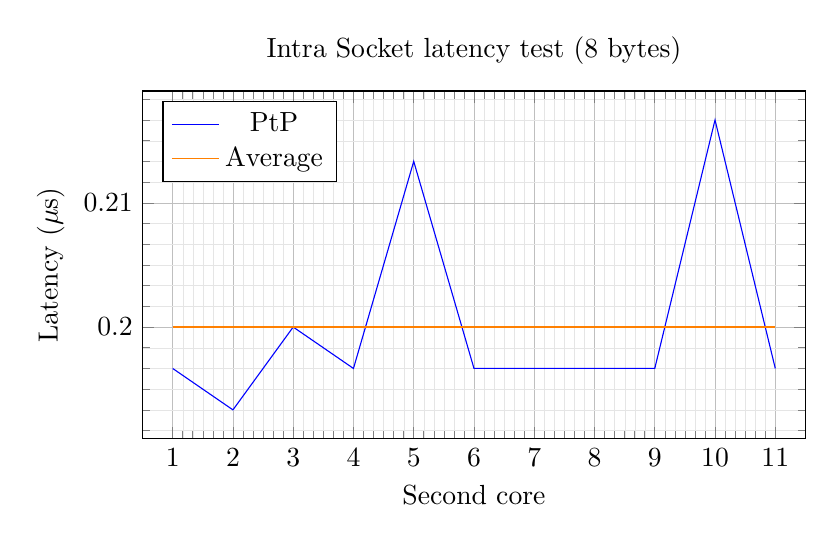
\begin{tikzpicture}
            \begin{axis}[
                title={Intra Socket latency test (8 bytes)},
                xlabel={Second core},
                ylabel={Latency ($\mu$s)},
                legend pos=north west,
                grid=both,
                grid style={line width=.1pt, draw=gray!20},
                major grid style={line width=.2pt,draw=gray!50},
                minor tick num=5,
                xtick={1, 2, 3, 4, 5, 6, 7, 8, 9, 10, 11},
                % xmode=log,
                % log basis x={2},
                % ymin=0,
                xmin=0.5,
                xmax=11.5,
                % xmax=100,
                % ytick={0, 50, 100, 150, 200, 250, 300, 350, 400},
                width=10cm,
                height=6cm,
                % cycle list name=color list,
            ]
            
            % x = [0,1,...,11]
            % y = [1.23599500e+04 1.96666667e-01 1.93333333e-01 2.00000000e-01 1.96666667e-01 2.13333333e-01 1.96666667e-01 1.96666667e-01 1.96666667e-01 1.96666667e-01 2.16666667e-01 1.96666667e-01]
            % avg = 0.19999999999999998
            % Blue line: Real
            \addplot[
                color=blue,
                mark=none,
                ]
                coordinates {
                (1, 0.196667)
                (2, 0.193333)
                (3, 0.200000)
                (4, 0.196667)
                (5, 0.213333)
                (6, 0.196667)
                (7, 0.196667)
                (8, 0.196667)
                (9, 0.196667)
                (10, 0.216667)
                (11, 0.196667)
                };
                \addlegendentry{PtP}
            
            % Orange line: Average
            \addplot[
                color=orange,
                mark=none,
                ]
                coordinates {
                (1, 0.19999999999999998)
                (11, 0.19999999999999998)
                };
                \addlegendentry{Average}
            
            \end{axis}
        \end{tikzpicture}
        }
    \end{figure}
    \begin{figure}[H]
        \centering
        \resizebox{0.45\textwidth}{!}{
        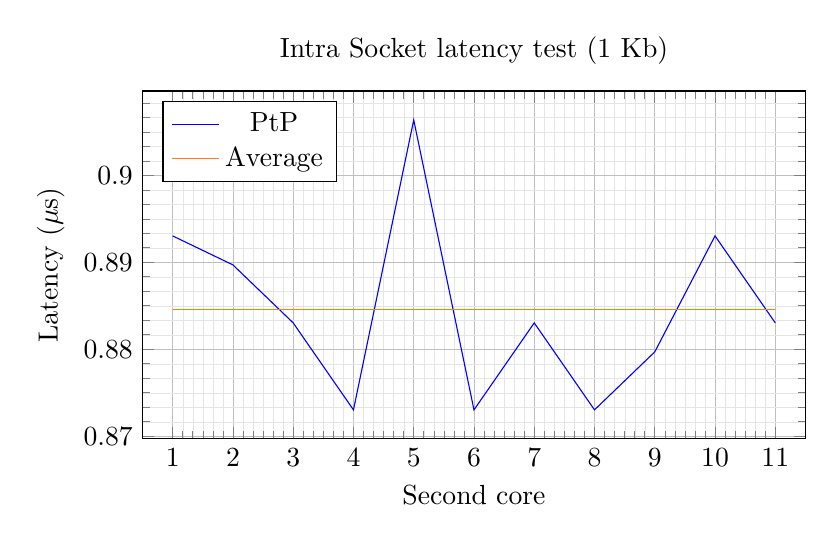
\begin{tikzpicture}
            \begin{axis}[
                title={Intra Socket latency test (1 Kb)},
                xlabel={Second core},
                ylabel={Latency ($\mu$s)},
                legend pos=north west,
                grid=both,
                grid style={line width=.1pt, draw=gray!20},
                major grid style={line width=.2pt,draw=gray!50},
                minor tick num=5,
                xtick={1, 2, 3, 4, 5, 6, 7, 8, 9, 10, 11},
                % xmode=log,
                % log basis x={2},
                % ymin=0,
                xmin=0.5,
                xmax=11.5,
                % xmax=100,
                % ytick={0, 50, 100, 150, 200, 250, 300, 350, 400},
                width=10cm,
                height=6cm,
                % cycle list name=color list,
            ]
            
            % x = [0,1,...,11]
            % y = [1.25343200e+04 8.93030303e-01 8.89696970e-01 8.83030303e-01 8.73030303e-01 9.06363636e-01 8.73030303e-01 8.83030303e-01 8.73030303e-01 8.79696970e-01 8.93030303e-01 8.83030303e-01 ]
            % avg = 0.8845454545454546
            % Blue line: Real
            \addplot[
                color=blue,
                mark=none,
                ]
                coordinates {
                (1, 0.893030)
                (2, 0.889697)
                (3, 0.883030)
                (4, 0.873030)
                (5, 0.906364)
                (6, 0.873030)
                (7, 0.883030)
                (8, 0.873030)
                (9, 0.879697)
                (10, 0.893030)
                (11, 0.883030)
                };
                \addlegendentry{PtP}
            
            % Orange line: Average
            \addplot[
                color=orange,
                mark=none,
                ]
                coordinates {
                (1, 0.8845454545454546)
                (11, 0.8845454545454546)
                };
                \addlegendentry{Average}
            
            \end{axis}
        \end{tikzpicture}
        }
    \end{figure}
    \begin{figure}[H]
        \centering
        \resizebox{0.45\textwidth}{!}{
        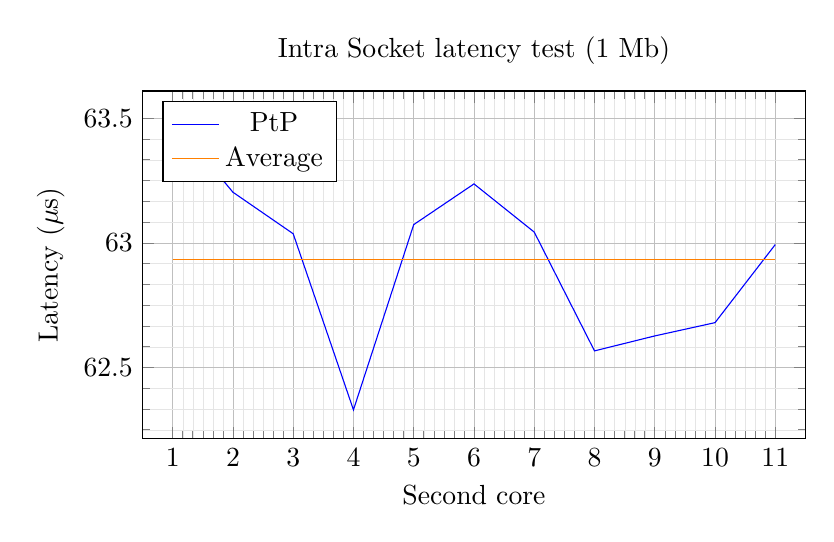
\begin{tikzpicture}
            \begin{axis}[
                title={Intra Socket latency test (1 Mb)},
                xlabel={Second core},
                ylabel={Latency ($\mu$s)},
                legend pos=north west,
                grid=both,
                grid style={line width=.1pt, draw=gray!20},
                major grid style={line width=.2pt,draw=gray!50},
                minor tick num=5,
                xtick={1, 2, 3, 4, 5, 6, 7, 8, 9, 10, 11},
                % xmode=log,
                % log basis x={2},
                % ymin=0,
                xmin=0.5,
                xmax=11.5,
                % xmax=100,
                % ytick={0, 50, 100, 150, 200, 250, 300, 350, 400},
                width=10cm,
                height=6cm,
                % cycle list name=color list,
            ]
            
            % x = [0,1,...,11]
            % y = [12189.89 63.4930303 63.2030303 63.03636364 62.32969697 63.0730303 63.23636364 63.0430303 62.56636364 62.62636364 62.67969697 62.9930303 ]
            % avg = 62.93454545454545
            % Blue line: Real
            \addplot[
                color=blue,
                mark=none,
                ]
                coordinates {
                (1, 63.4930303)
                (2, 63.2030303)
                (3, 63.03636364)
                (4, 62.32969697)
                (5, 63.0730303)
                (6, 63.23636364)
                (7, 63.0430303)
                (8, 62.56636364)
                (9, 62.62636364)
                (10, 62.67969697)
                (11, 62.9930303)
                };
                \addlegendentry{PtP}
            
            % Orange line: Average
            \addplot[
                color=orange,
                mark=none,
                ]
                coordinates {
                (1, 62.93454545454545)
                (11, 62.93454545454545)
                };
                \addlegendentry{Average}
            
            \end{axis}
        \end{tikzpicture}
        }
    \end{figure}
    The communication is the slowest when the second process is bound
    to the same core as the first process. We do not represet this
    value in the plot for readability reasons. Hereafter we report
    some further statistics:
    % Table
    \begin{table}[H]
        \centering
        \begin{tabular}{|c|c|c|c|}
            \hline
            \textbf{Message size} & \textbf{Average ($\mu$s)} & \textbf{Std ($\mu$s)} & \textbf{Std/Average} \\
            \hline
            8 bytes & 0.19 & 0.007 & 0.0362 \\
            1 Kb & 0.88 & 0.009 & 0.0111 \\
            1 Mb & 62.93 & 0.33 & 0.005 \\
            \hline
        \end{tabular}
    \end{table}
    As we can see, the absolute variability of the latency increases
    with the message size. However, if we consider the relative
    variability, we can see that the latency is more stable for larger
    messages.
    Finally, we analyze all the tested message sizes averaging the
    latencies among each core combination.
    \begin{figure}[H]
        \centering
        \resizebox{0.45\textwidth}{!}{
        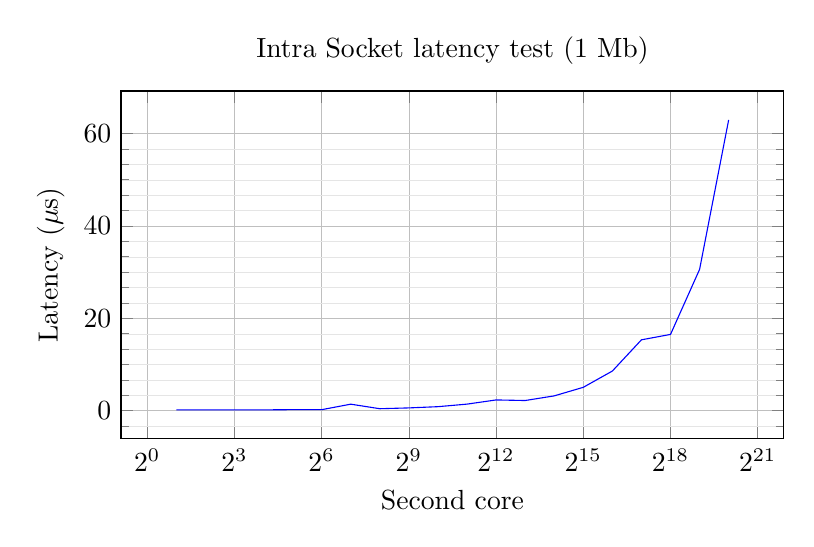
\begin{tikzpicture}
            \begin{axis}[
                title={Intra Socket latency test (1 Mb)},
                xlabel={Second core},
                ylabel={Latency ($\mu$s)},
                legend pos=north west,
                grid=both,
                grid style={line width=.1pt, draw=gray!20},
                major grid style={line width=.2pt,draw=gray!50},
                minor tick num=5,
                % xtick={1, 2, 3, 4, 5, 6, 7, 8, 9, 10, 11},
                xmode=log,
                log basis x={2},
                % ymin=0,
                % xmin=0.5,
                % xmax=11.5,
                % xmax=100,
                % ytick={0, 50, 100, 150, 200, 250, 300, 350, 400},
                width=10cm,
                height=6cm,
                % cycle list name=color list,
            ]
            
            % x = [[      2,       4,       8,      16,      32,      64,     128,     256,           512,    1024,    2048,    4096,    8192,   16384,   32768,   65536, 131072,  262144,  524288, 1048576]
            % y = [ 0.19181818  0.19636364  0.2         0.19090909  0.24090909  0.23272727  1.42545455  0.44272727  0.61818182  0.88454545  1.43636364  2.34272727  2.21636364  3.22181818  5.07454545  8.59727273 15.35272727 16.52272727 30.58909091 62.93454545]
            % Blue line: Real
            \addplot[
                color=blue,
                mark=none,
                ]
                coordinates {
                (2, 0.19181818)
                (4, 0.19636364)
                (8, 0.2)
                (16, 0.19090909)
                (32, 0.24090909)
                (64, 0.23272727)
                (128, 1.42545455)
                (256, 0.44272727)
                (512, 0.61818182)
                (1024, 0.88454545)
                (2048, 1.43636364)
                (4096, 2.34272727)
                (8192, 2.21636364)
                (16384, 3.22181818)
                (32768, 5.07454545)
                (65536, 8.59727273)
                (131072, 15.35272727)
                (262144, 16.52272727)
                (524288, 30.58909091)
                (1048576, 62.93454545)
                };
            
            \end{axis}
        \end{tikzpicture}
        }
    \end{figure}
    Even with the significant increase in the latency for larger messages,
    its growth is not exponential. Meaning that the increment in the 
    latency is not proportional to the message size.


\subsubsection{Intra-Node}
    In this test we bind the two processes to different sockets. We fix
    the first process to socket 0 core 0 and the second process to socket
    1 core 0. We vary the second process from core 0 to core 3, 6, and 10.
    We again expect the latency to be stable across the different cores and
    this is the reason we tested only four of them. Since we have less test
    points we directly report a table.
    % Table
    \begin{table}[H]
        \centering
        \begin{tabular}{|c|c|c|c|}
            \hline
            \textbf{Message size} & \textbf{Average ($\mu$s)} & \textbf{Std ($\mu$s)} & \textbf{Std/Average} \\
            \hline
            8 bytes & 0.405 & 0.005 & 0.0123 \\
            1 Kb & 1.9175 & 0.0217 & 0.0113 \\
            1 Mb & 63.6575 & 0.8918 & 0.0140 \\
            \hline
        \end{tabular}
    \end{table}
    This time we observe a different behaviour in the variability-to-average
    ratio. Instead of decreasing as in the previous test, it stays almost
    constant around an average of $0.0125$.

\subsubsection{Intra-Cluster}
    Finally we test the latency between two processes on different nodes.
    We test the following combinations:
    \begin{itemize}
        \item N0 S0 C0 $\leftrightarrow$ N1 S0 C0
        \item N0 S0 C0 $\leftrightarrow$ N1 S1 C0
        \item N0 S1 C0 $\leftrightarrow$ N1 S0 C0
        \item N0 S1 C0 $\leftrightarrow$ N1 S1 C0
    \end{itemize}
    Again we report the results in a table.
    \begin{table}[H]
        \centering
        \begin{tabular}{|c|c|c|c|}
            \hline
            \textbf{Message size} & \textbf{Average ($\mu$s)} & \textbf{Std ($\mu$s)} & \textbf{Std/Average} \\
            \hline
            8 bytes & 1.1250 & 0.0622 & 0.0553 \\
            1 Kb & 1.9550 & 0.1484 & 0.0759 \\
            1 Mb & 94.2250 & 0.3829 & 0.0041 \\
            \hline
        \end{tabular}
    \end{table}
    This time we observe again a different behaviour in the variability-to-average
    ratio. It increases when considering low values of the message size and
    then drops for larger values becoming more and more stable.

\subsection{Broadcast}
    The broadcast operation is used to send a message from the root
    process to all the other processes in the communicator. 
    This is useful when the root process has a block of data that needs
    to be entirely copied to all the other processes. \\
    The parameters for the tests are:
    \begin{itemize}
        \item iterations: 1000
        \item warmup: 100
        \item algorithms: basic linear, chain, binary tree
        \item message size: 1byte $\rightarrow$ 1 Mb
        \item number of processes: $2, 4, \dots, 48$
    \end{itemize}
    Again we repeat the tests intra-socket, intra-node, and intra-cluster.
\subsubsection{Intra-Socket}
    Mapping by core, we perform the broadcast operation between multiple
    processes on the same socket. The average latencies are reported in
    plot below.
    % Basic Linear
    \begin{figure}[H]
        \centering
        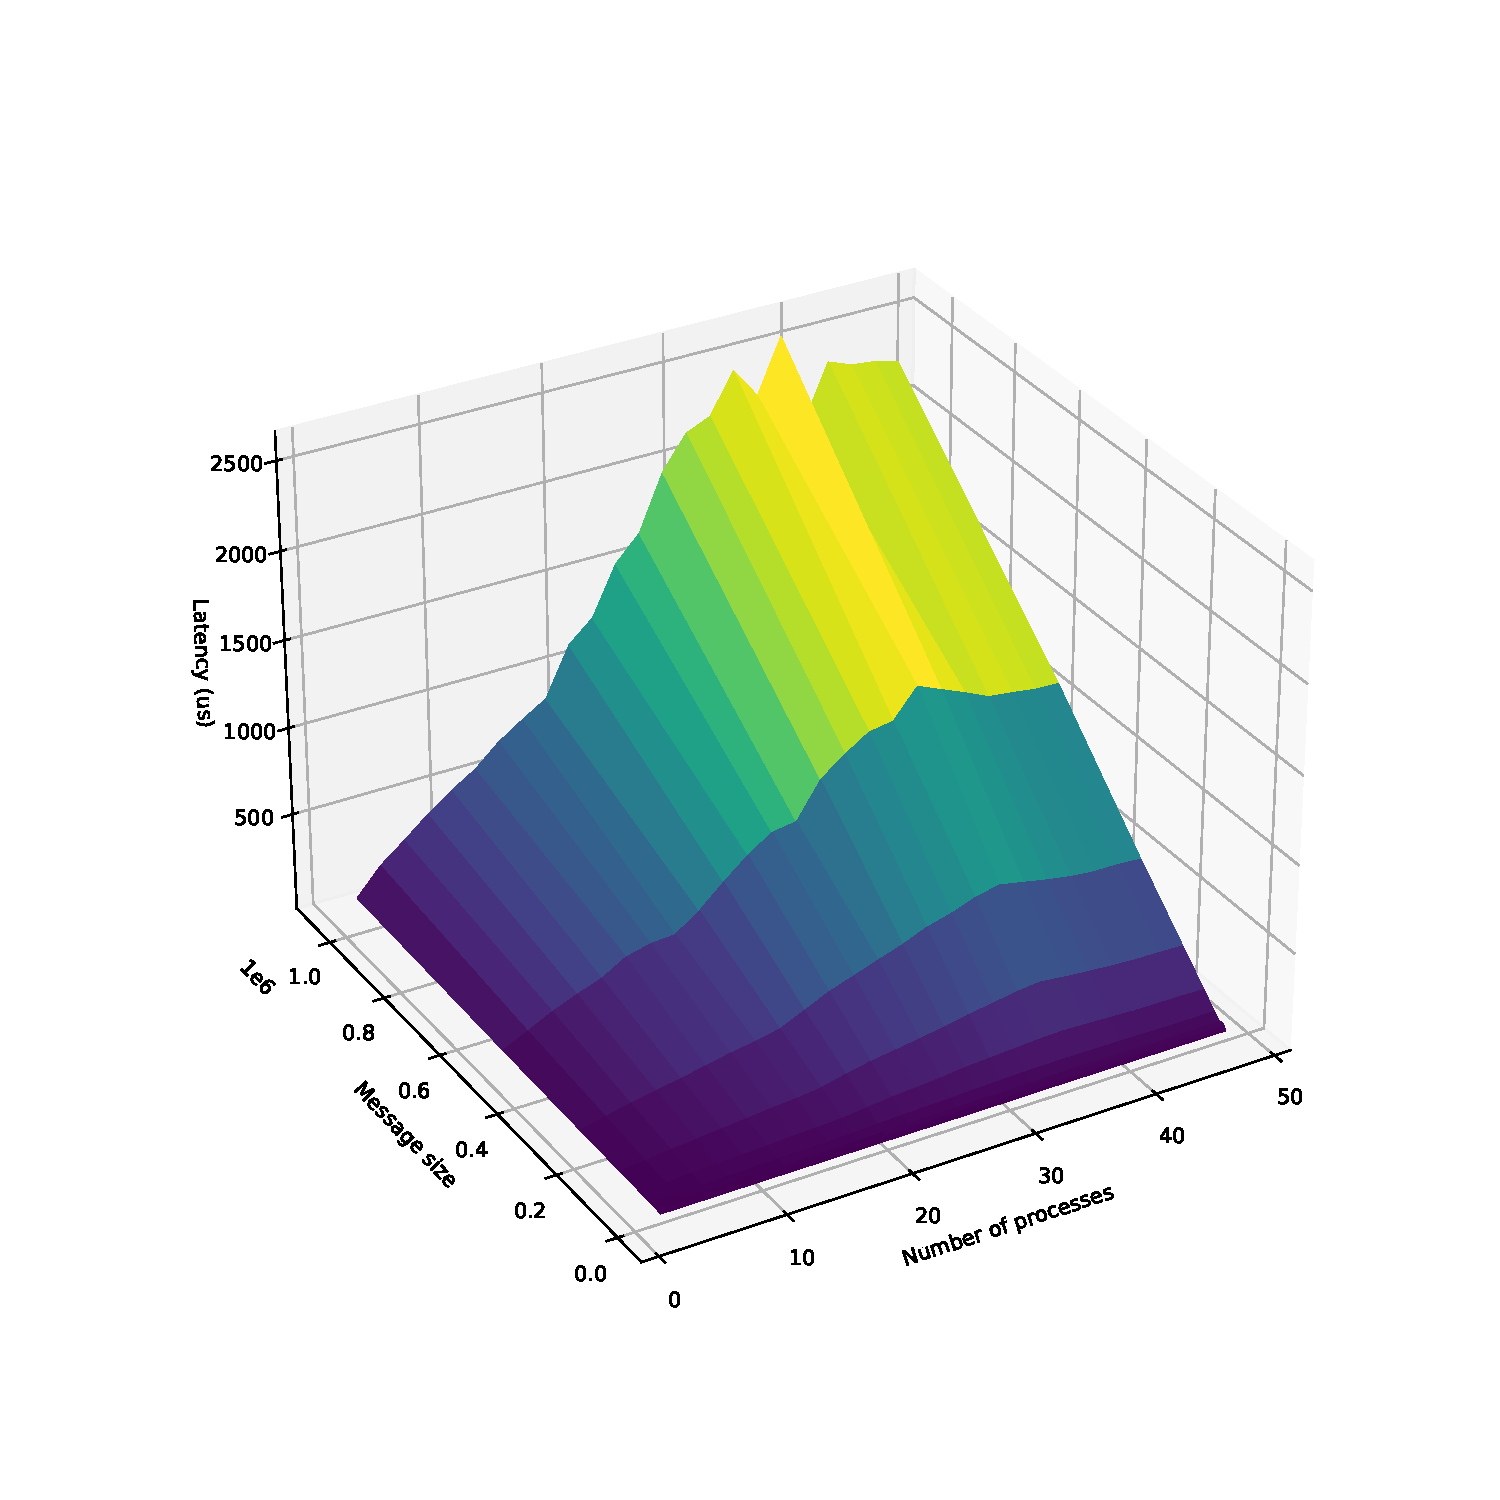
\includegraphics[
            width=0.45\textwidth,
            clip,
            trim=0 3cm 0 4.5cm
        ]{figures/bcast_socket_alg1.pdf}
        \caption{Intra-Socket broadcast latency (basic linear)}
    \end{figure}
    % Chain
    \begin{figure}[H]
        \centering
        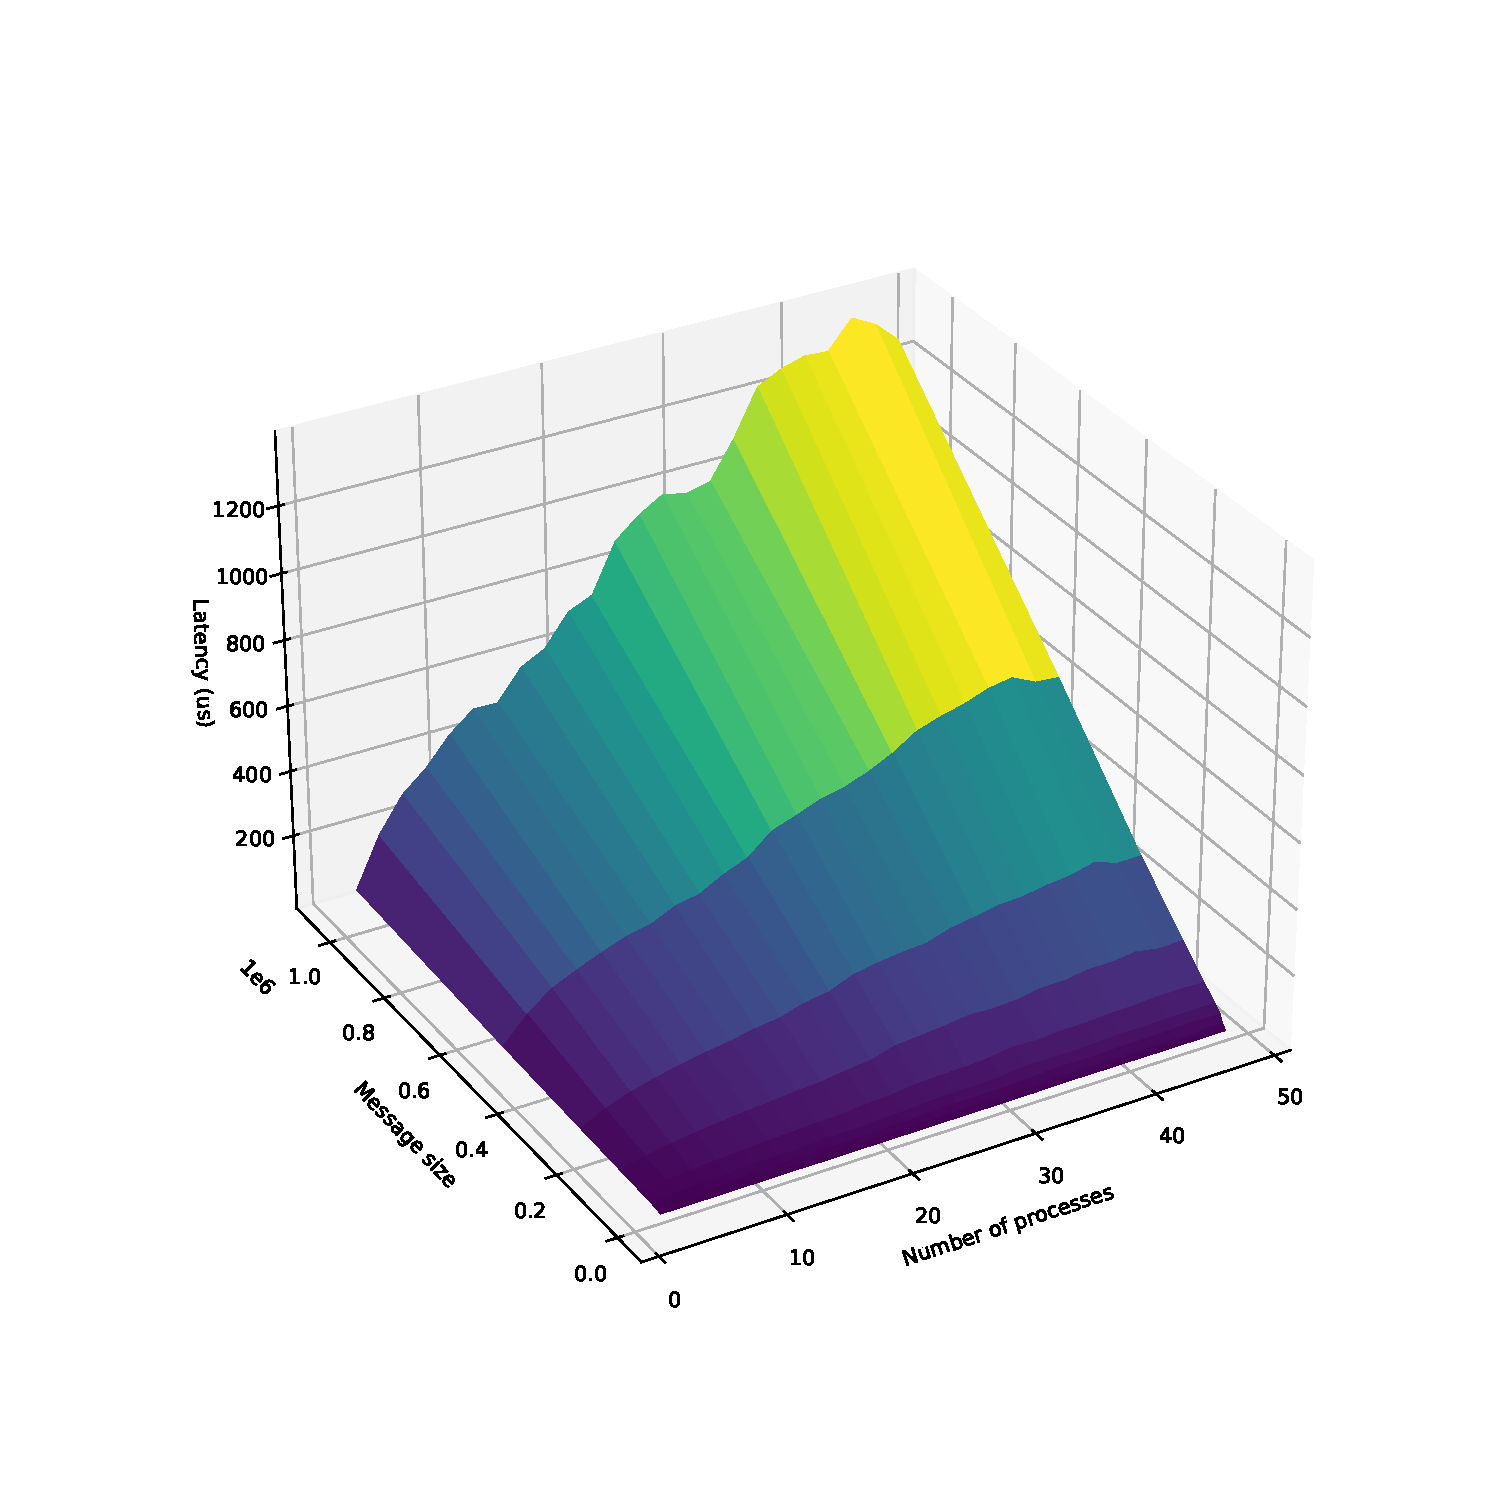
\includegraphics[
            width=0.45\textwidth,
            clip,
            trim=0 3cm 0 4.5cm
        ]{figures/bcast_socket_alg2.pdf}
        \caption{Intra-Socket broadcast latency (chain)}
    \end{figure}
    % Binary Tree
    \begin{figure}[H]
        \centering
        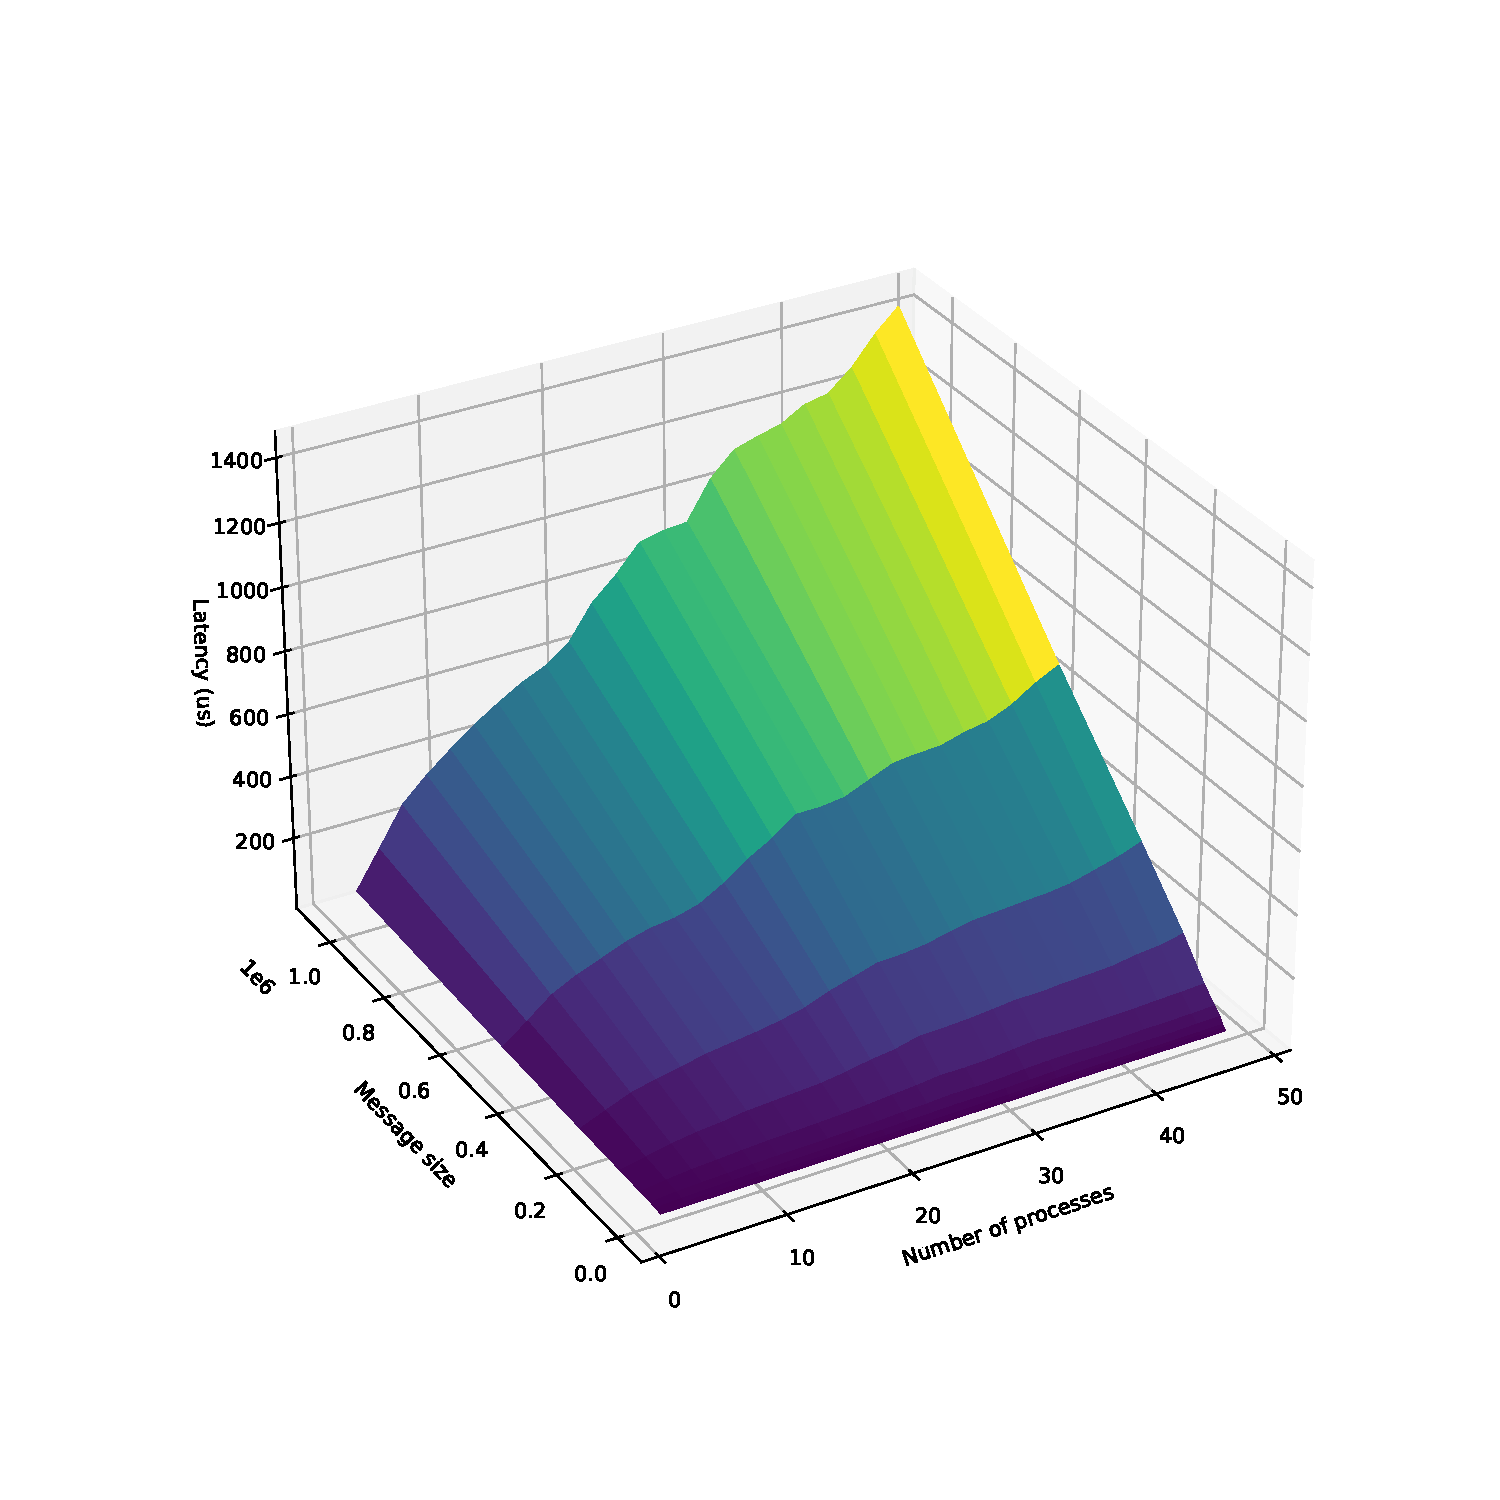
\includegraphics[
            width=0.45\textwidth,
            clip,
            trim=0 3cm 0 4.5cm
        ]{figures/bcast_socket_alg5.pdf}
        \caption{Intra-Socket broadcast latency (binary tree)}
    \end{figure}
\subsubsection{Intra-Node}
    Mapping by socket, we perform the broadcast operation between multiple
    processes on different sockets. The average latencies are reported in
    plot below.
    % Basic Linear
    \begin{figure}[H]
        \centering
        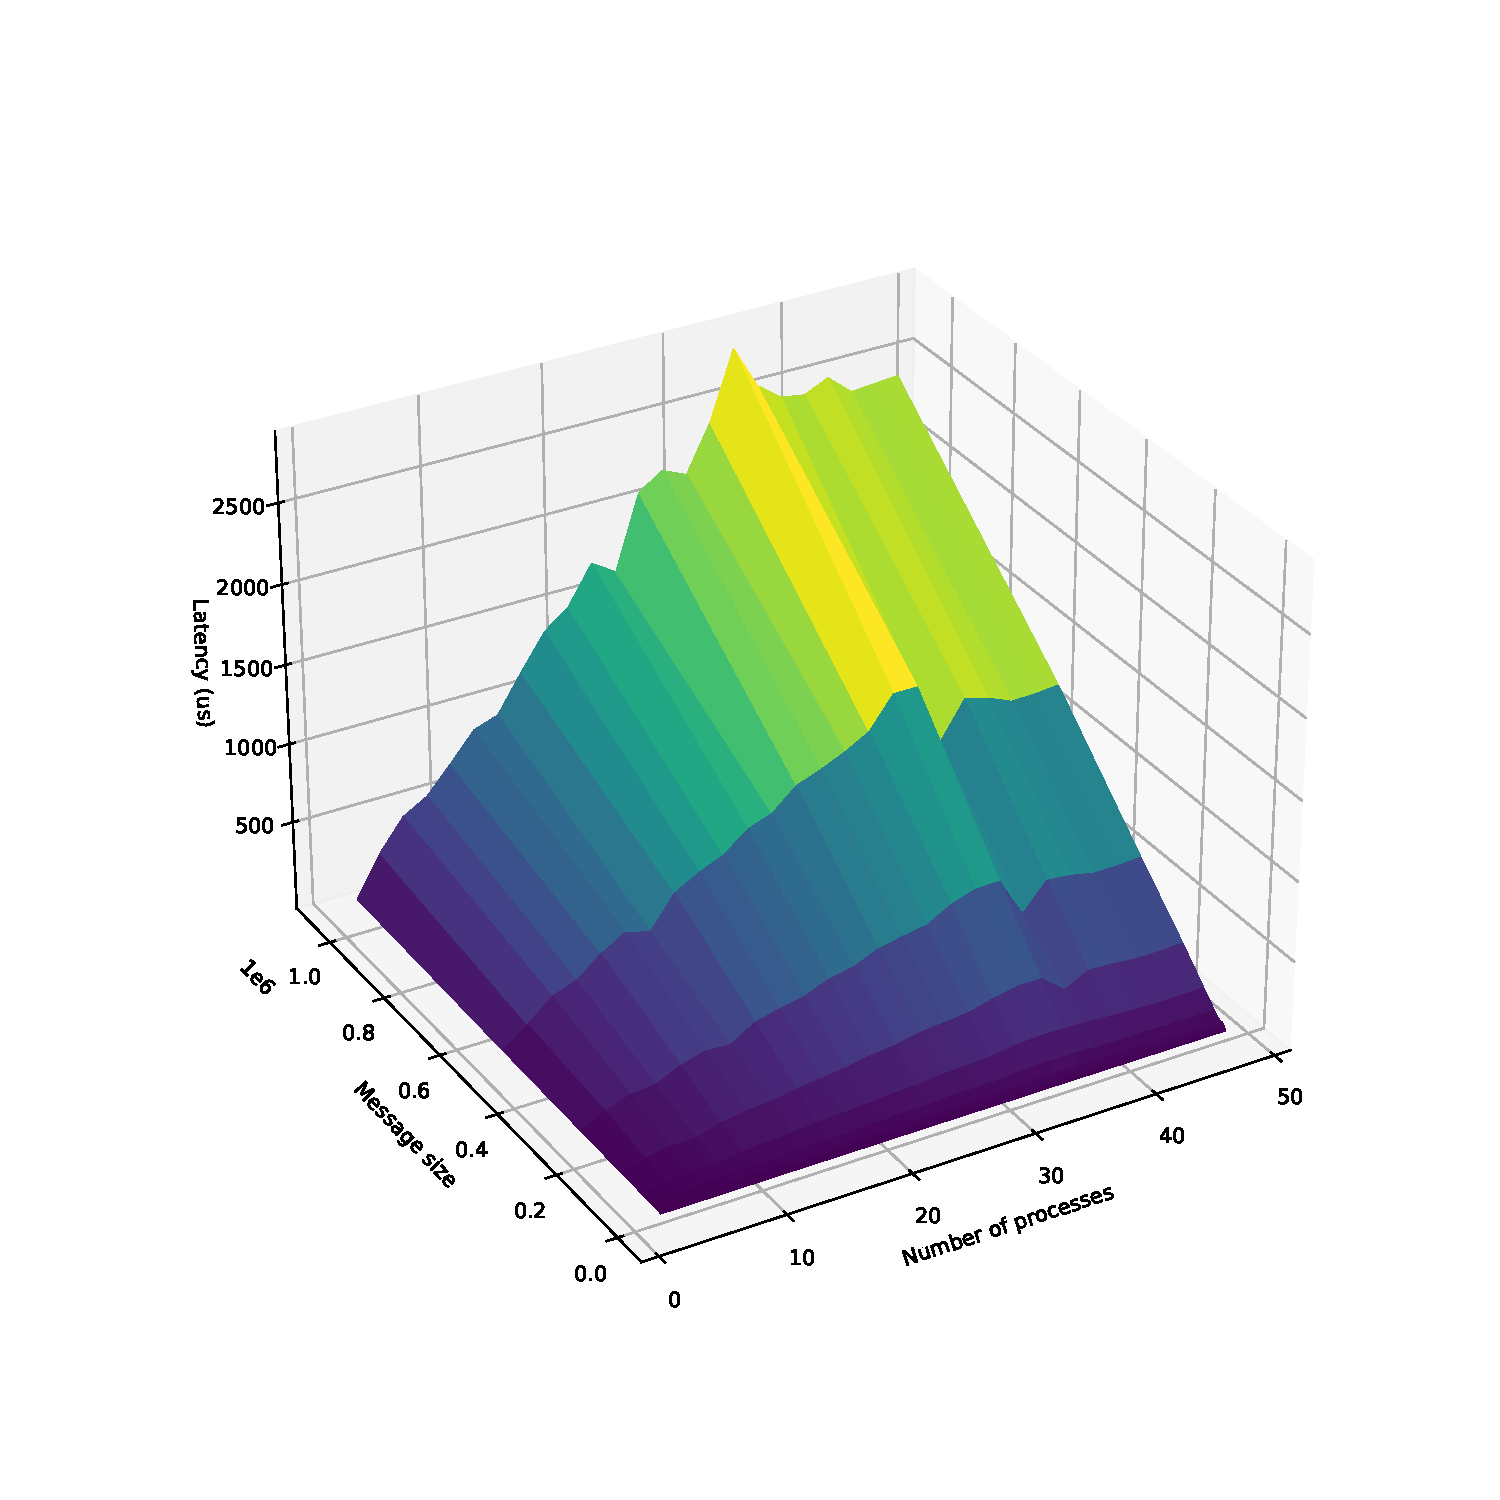
\includegraphics[
            width=0.45\textwidth,
            clip,
            trim=0 3cm 0 4.5cm
        ]{figures/bcast_node_alg1.pdf}
        \caption{Intra-Node broadcast latency (basic linear)}
    \end{figure}
    % Chain
    \begin{figure}[H]
        \centering
        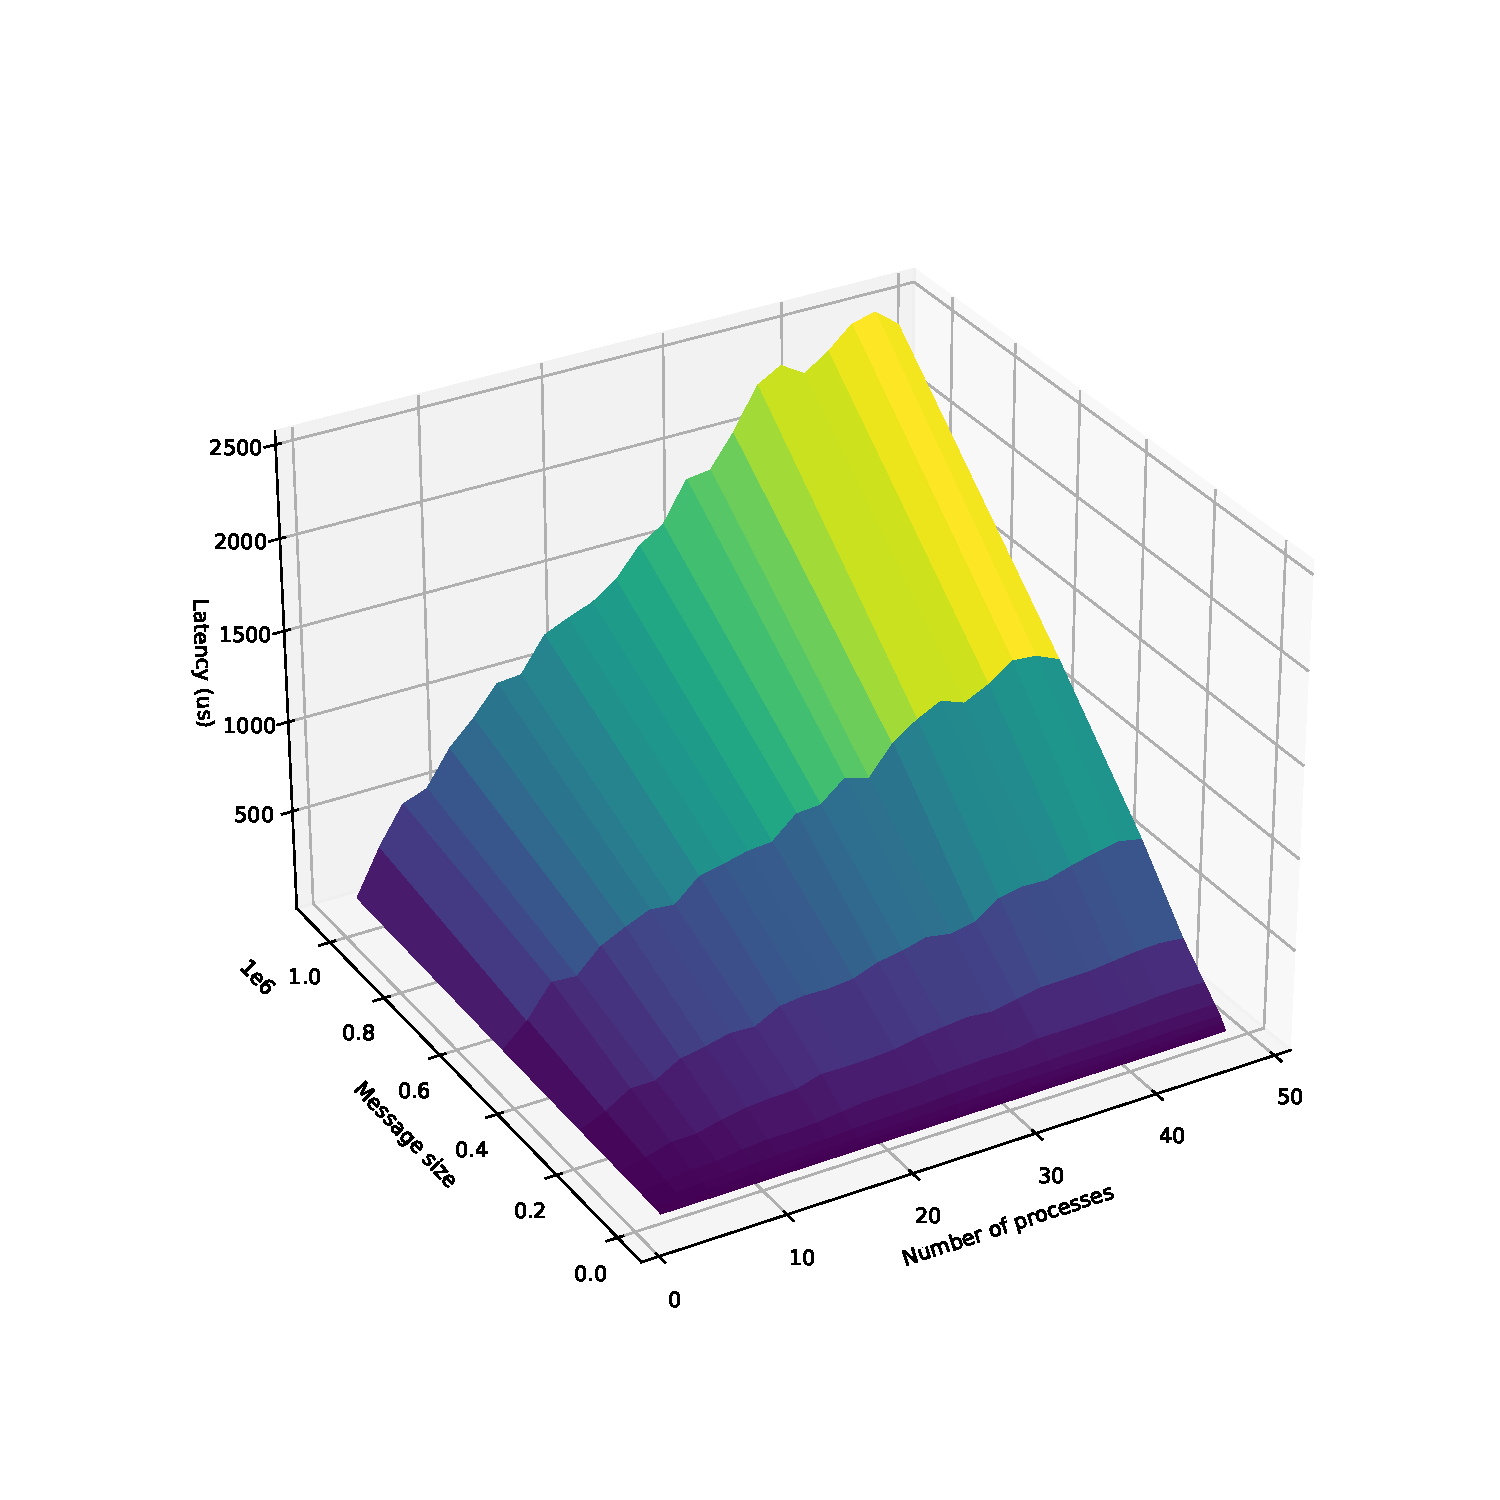
\includegraphics[
            width=0.45\textwidth,
            clip,
            trim=0 3cm 0 4.5cm
        ]{figures/bcast_node_alg2.pdf}
        \caption{Intra-Node broadcast latency (chain)}
    \end{figure}
    % Binary Tree
    \begin{figure}[H]
        \centering
        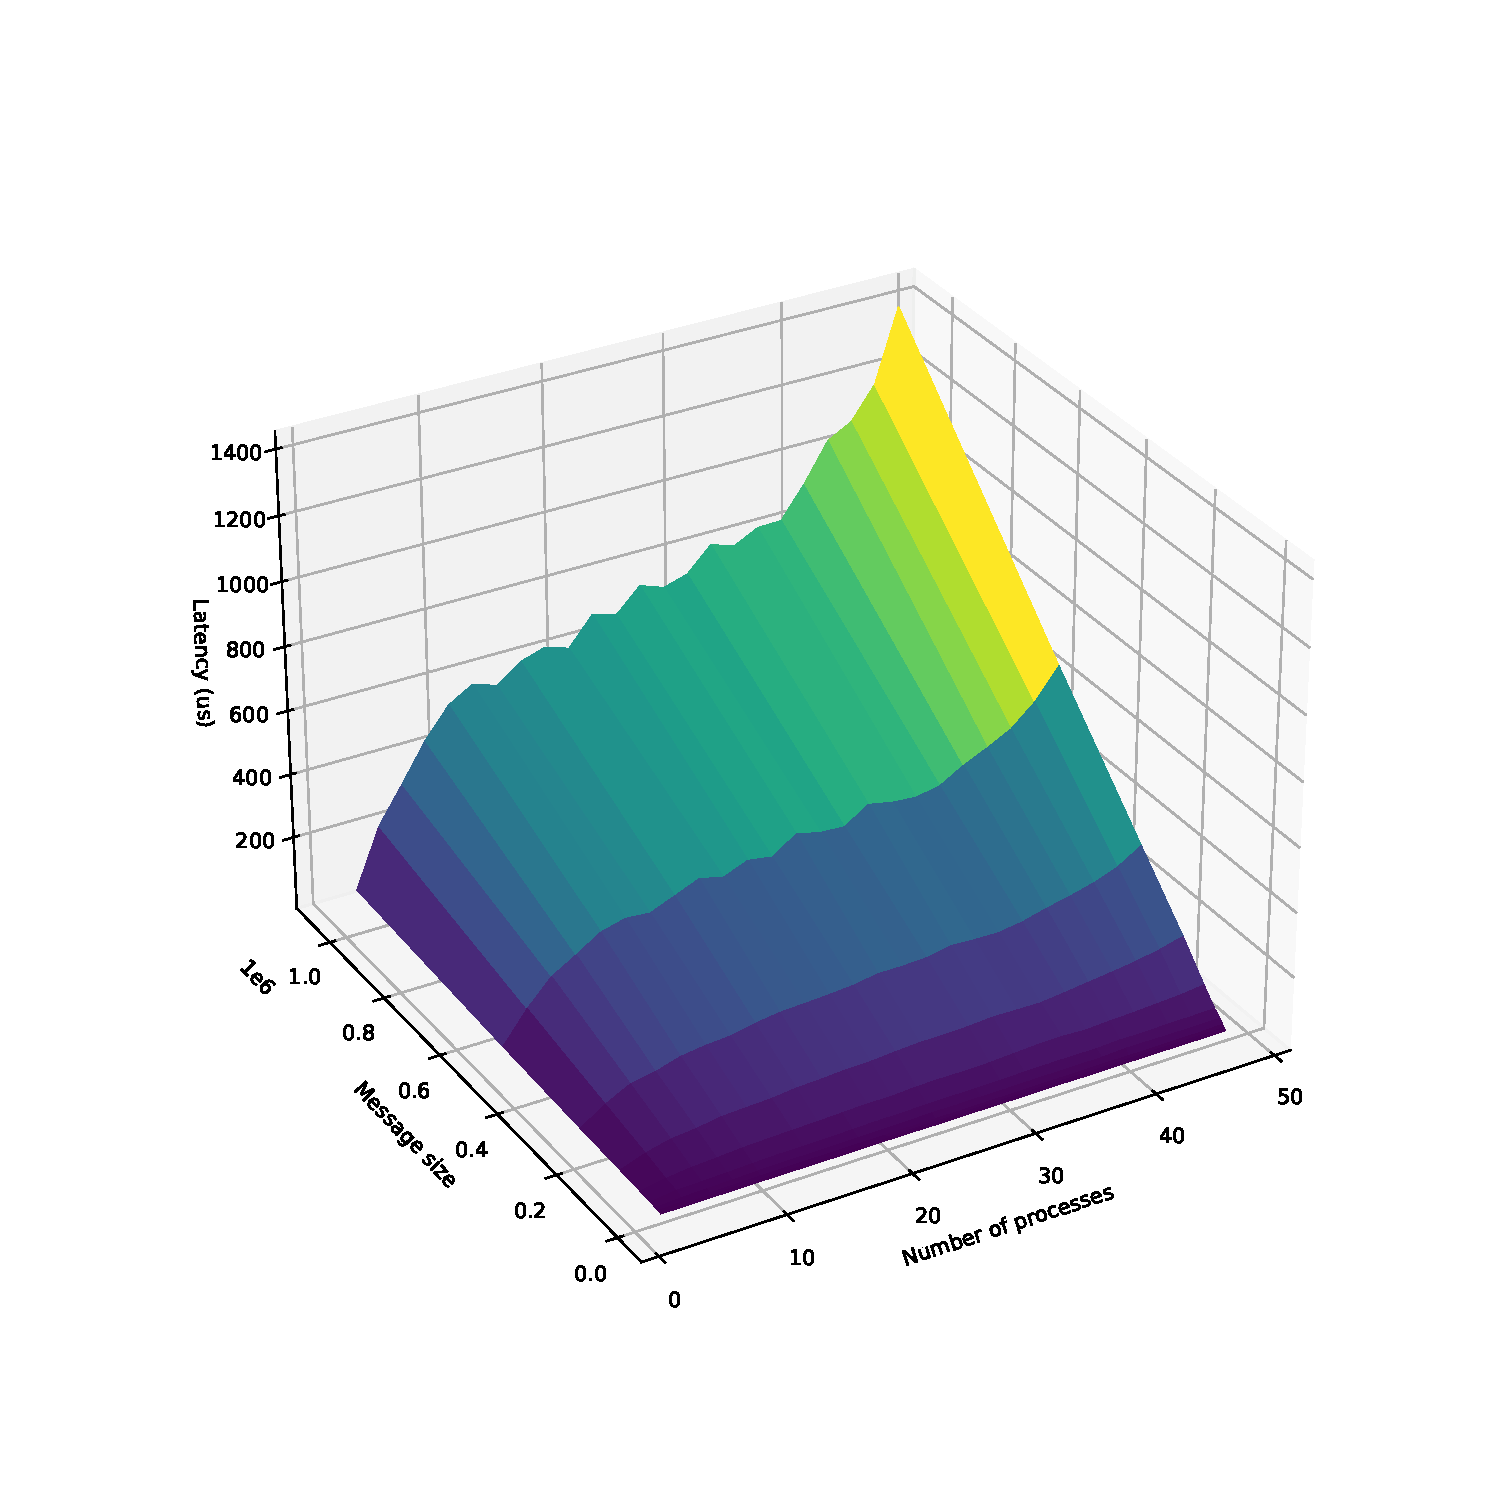
\includegraphics[
            width=0.45\textwidth,
            clip,
            trim=0 3cm 0 4.5cm
        ]{figures/bcast_node_alg5.pdf}
        \caption{Intra-Node broadcast latency (binary tree)}
    \end{figure}
\subsubsection{Intra-Cluster}
    Mapping by node, we perform the broadcast operation between multiple
    processes on different nodes. The average latencies are reported in
    plot below.
    % Basic Linear
    \begin{figure}[H]
        \centering
        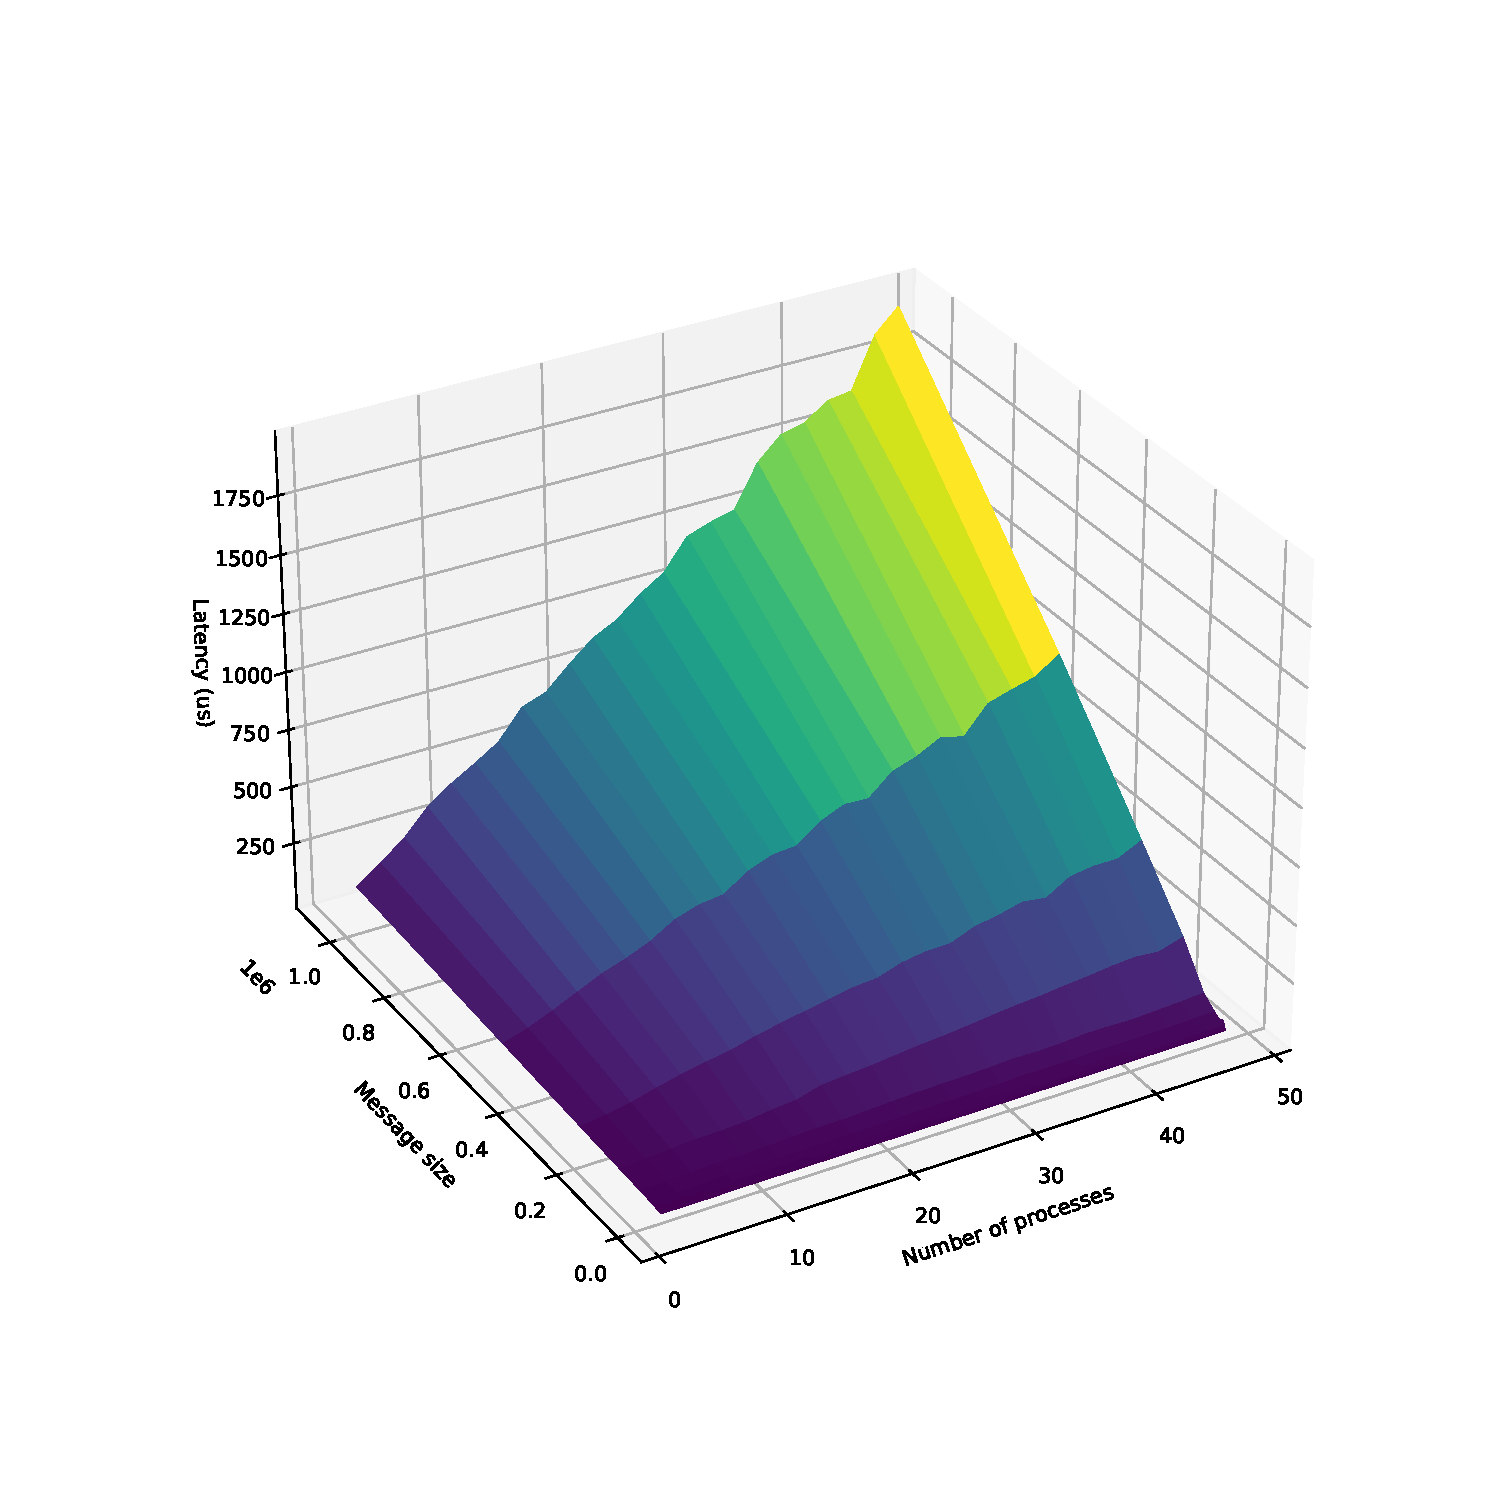
\includegraphics[
            width=0.45\textwidth,
            clip,
            trim=0 3cm 0 4.5cm
        ]{figures/bcast_cluster_alg1.pdf}
        \caption{Intra-Cluster broadcast latency (basic linear)}
    \end{figure}
    % Chain
    \begin{figure}[H]
        \centering
        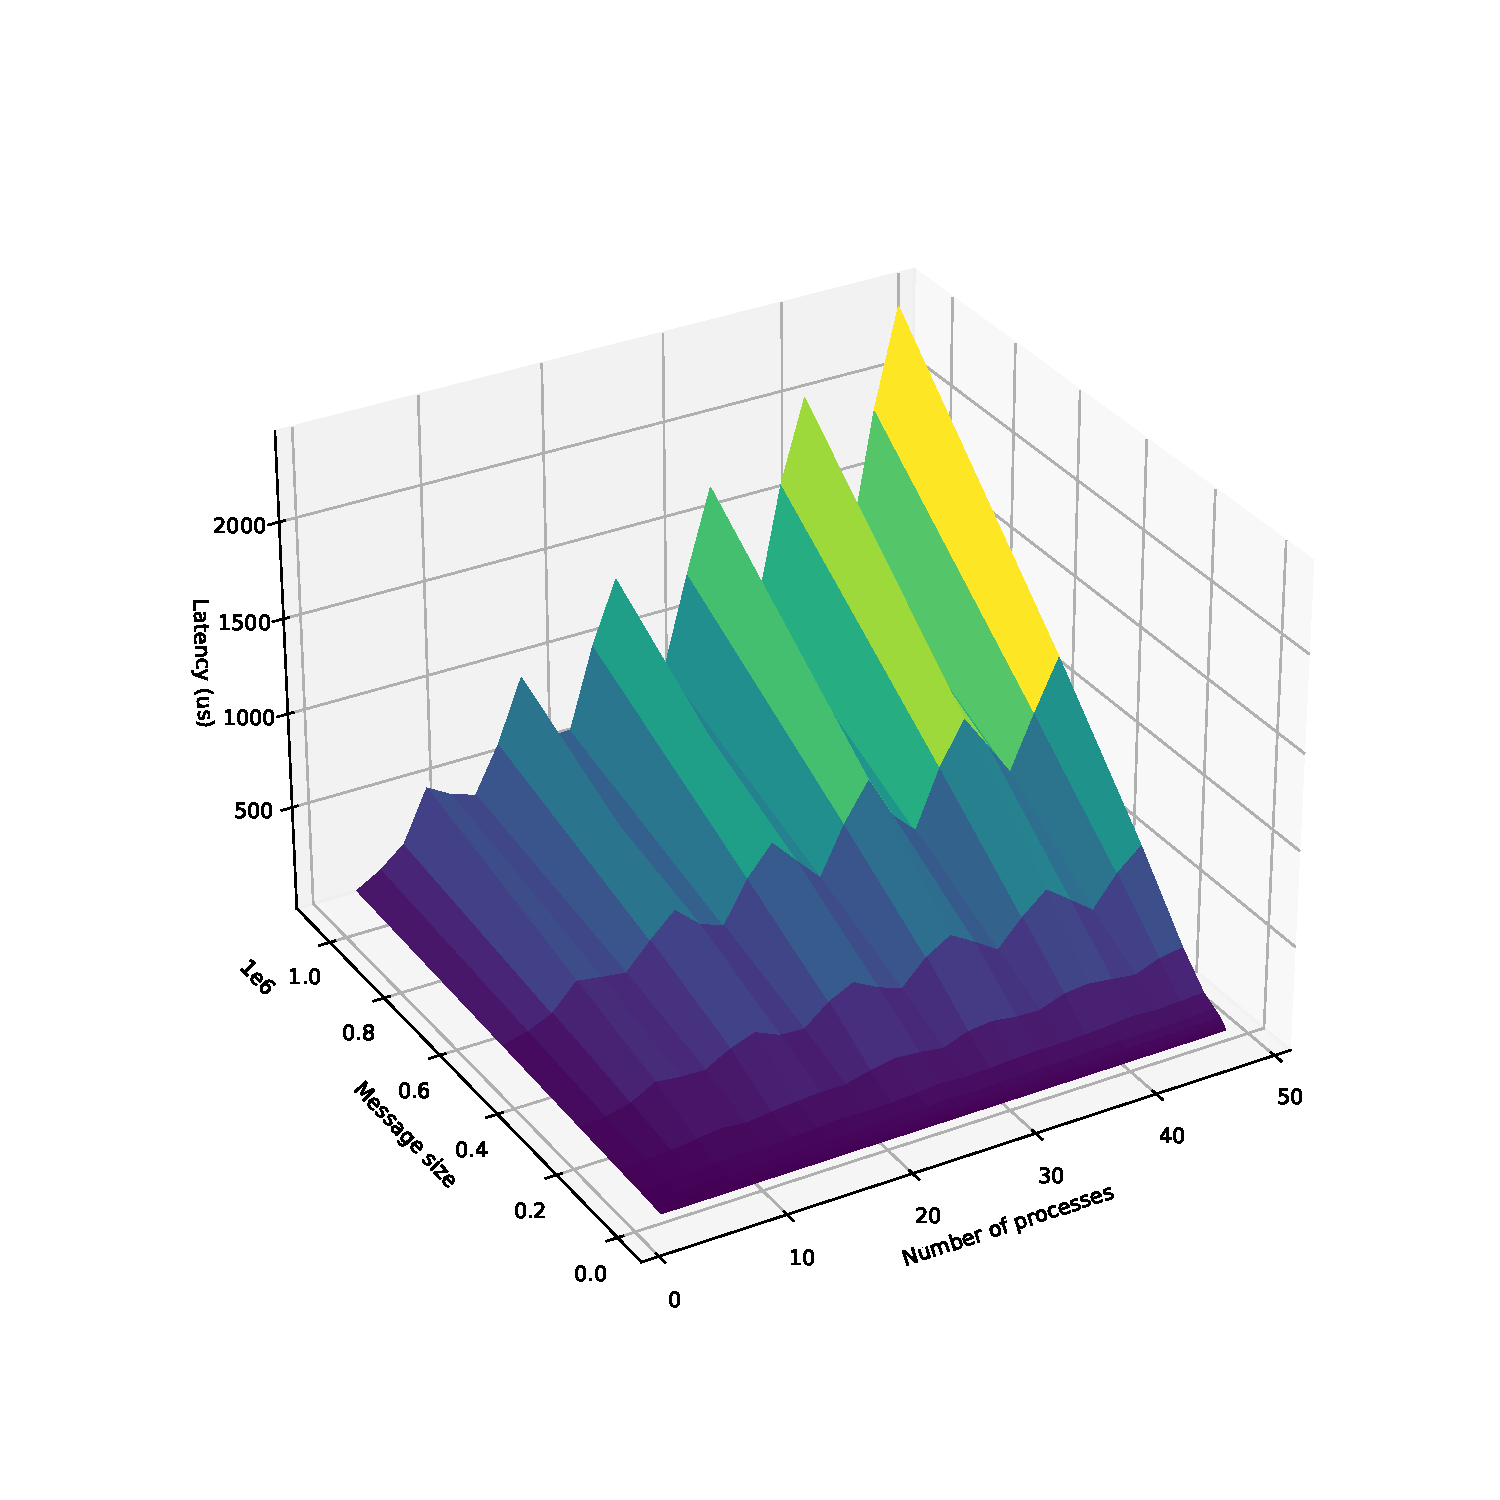
\includegraphics[
            width=0.45\textwidth,
            clip,
            trim=0 3cm 0 4.5cm
        ]{figures/bcast_cluster_alg2.pdf}
        \caption{Intra-Cluster broadcast latency (chain)}
    \end{figure}
    % Binary Tree
    \begin{figure}[H]
        \centering
        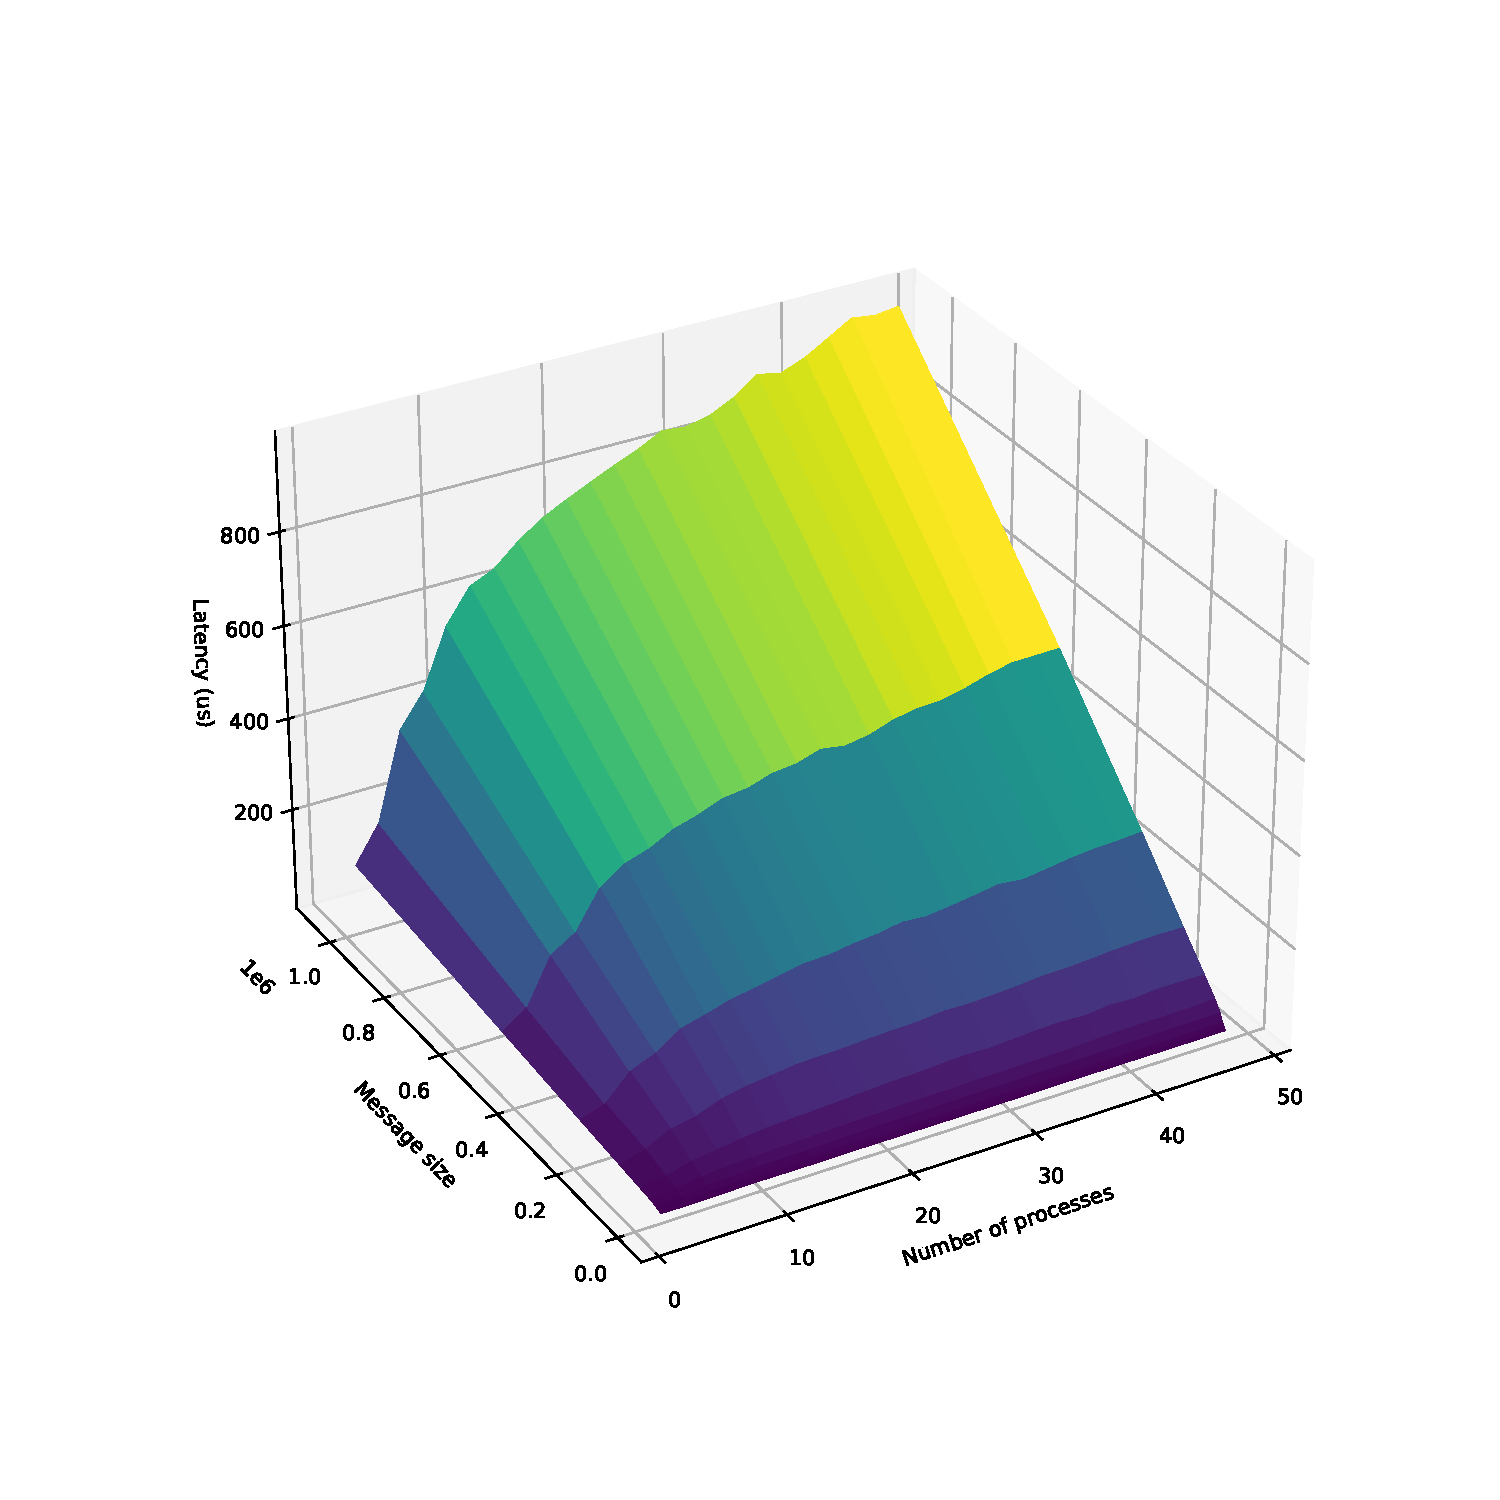
\includegraphics[
            width=0.45\textwidth,
            clip,
            trim=0 3cm 0 4.5cm
        ]{figures/bcast_cluster_alg5.pdf}
        \caption{Intra-Cluster broadcast latency (binary tree)}
    \end{figure}

    

\subsection{Scatter}
    The scatter operation is similar to broadcast, but instead of sending
    the entire message to all the other processes, the root process
    sends a different chunks of the message to each process. This is useful
    when the root process has a block of data that needs to be divided
    among all the other processes.
    The parameters for the tests are:
    \begin{itemize}
        \item iterations: 1000
        \item warmup: 100
        \item algorithms: basic linear, binomial
        \item message size: 1byte $\rightarrow$ 1 Mb
        \item number of processes: $2, 4, \dots, 48$
    \end{itemize}
    Once more, we repeat the tests intra-socket, intra-node, and intra-cluster.
\subsubsection{Intra-Socket}
    Mapping by core, we perform the scatter operation between multiple
    processes on the same socket. The average latencies are reported in
    plot below.
    % Basic Linear
    \begin{figure}[H]
        \centering
        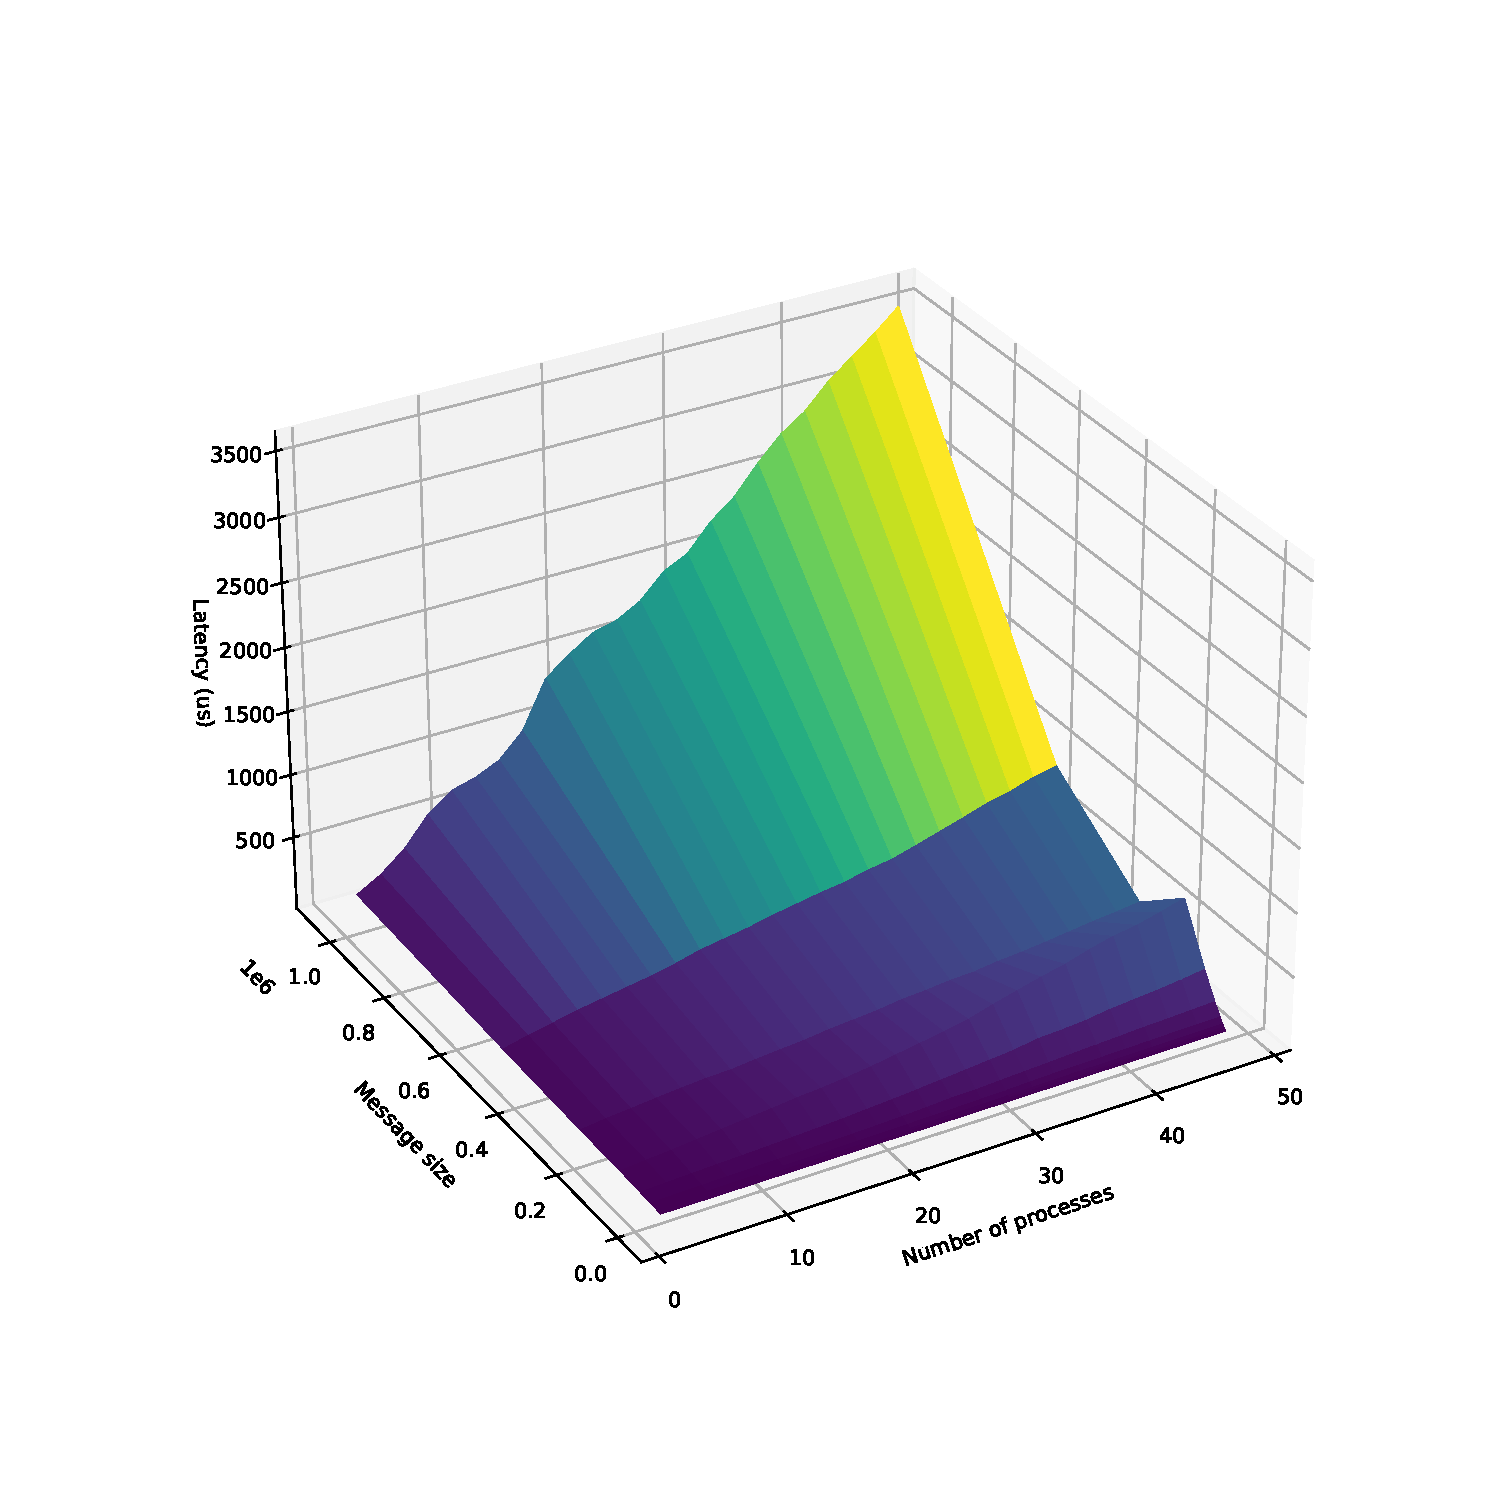
\includegraphics[
            width=0.45\textwidth,
            clip,
            trim=0 3cm 0 4.5cm
        ]{figures/scat_socket_alg1.pdf}
        \caption{Intra-Socket scatter latency (basic linear)}
    \end{figure}
    % Binomial
    \begin{figure}[H]
        \centering
        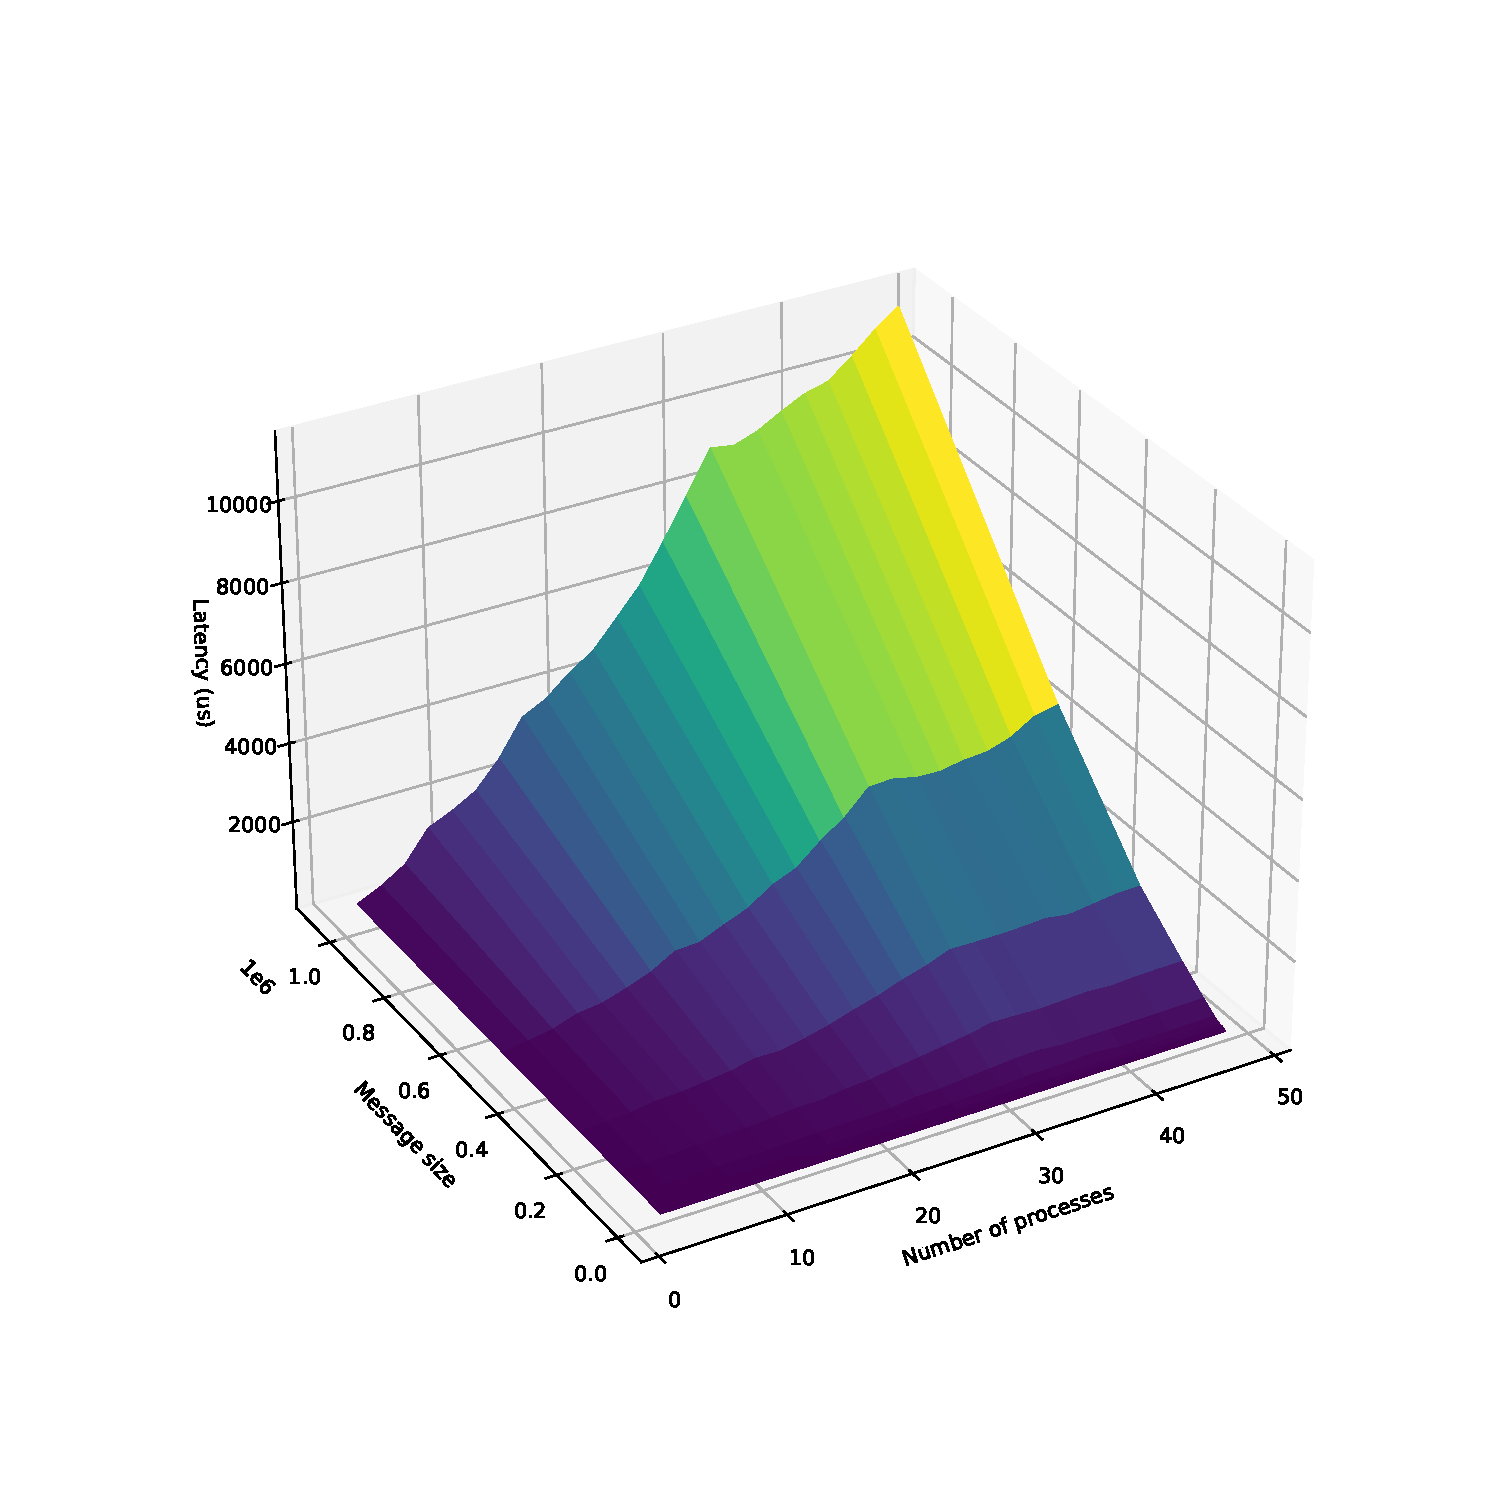
\includegraphics[
            width=0.45\textwidth,
            clip,
            trim=0 3cm 0 4.5cm
        ]{figures/scat_socket_alg2.pdf}
        \caption{Intra-Socket scatter latency (binomial)}
    \end{figure}
\subsubsection{Intra-Node}
    Mapping by socket, we perform the scatter operation between multiple
    processes on different sockets. The average latencies are reported in
    plot below.
    % Basic Linear
    \begin{figure}[H]
        \centering
        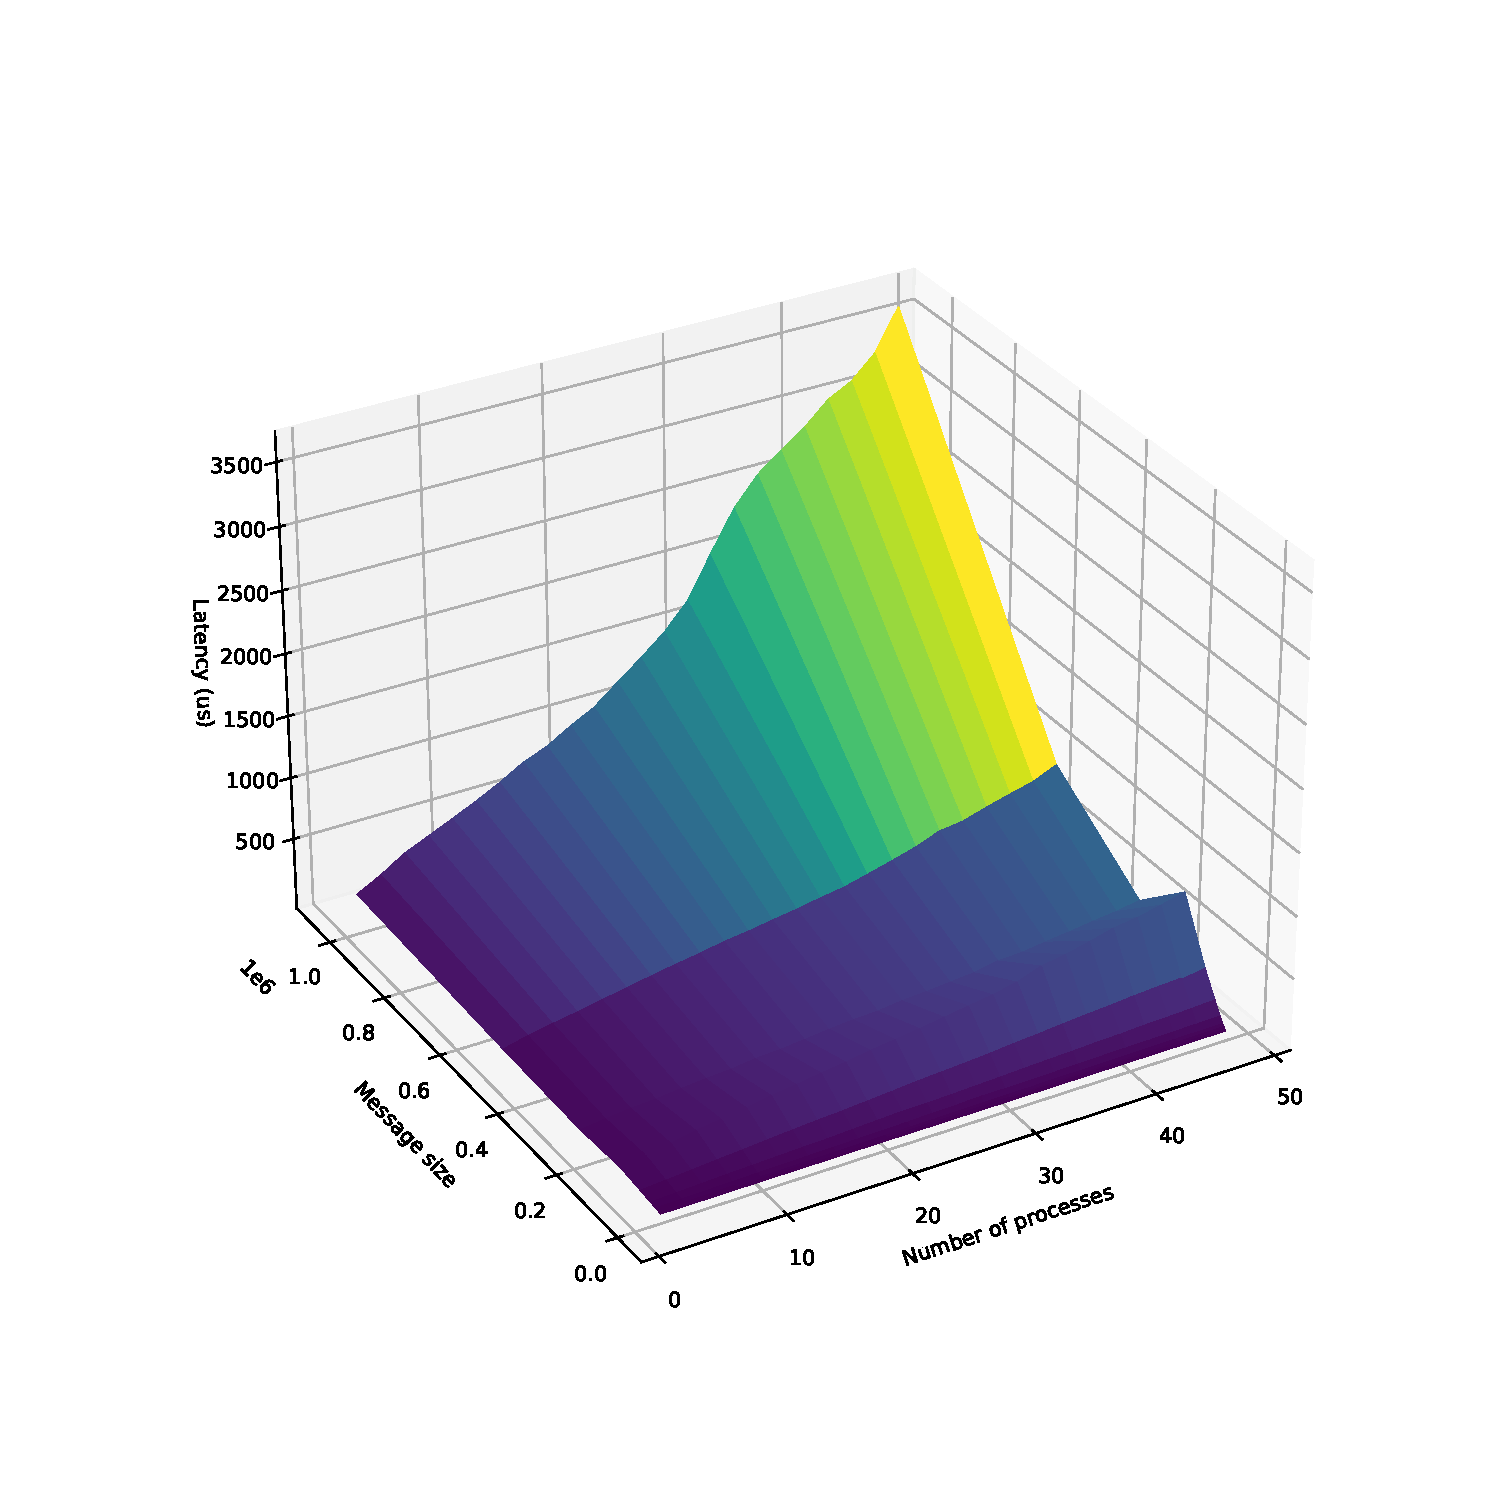
\includegraphics[
            width=0.45\textwidth,
            clip,
            trim=0 3cm 0 4.5cm
        ]{figures/scat_node_alg1.pdf}
        \caption{Intra-Node scatter latency (basic linear)}
    \end{figure}
    % Binomial
    \begin{figure}[H]
        \centering
        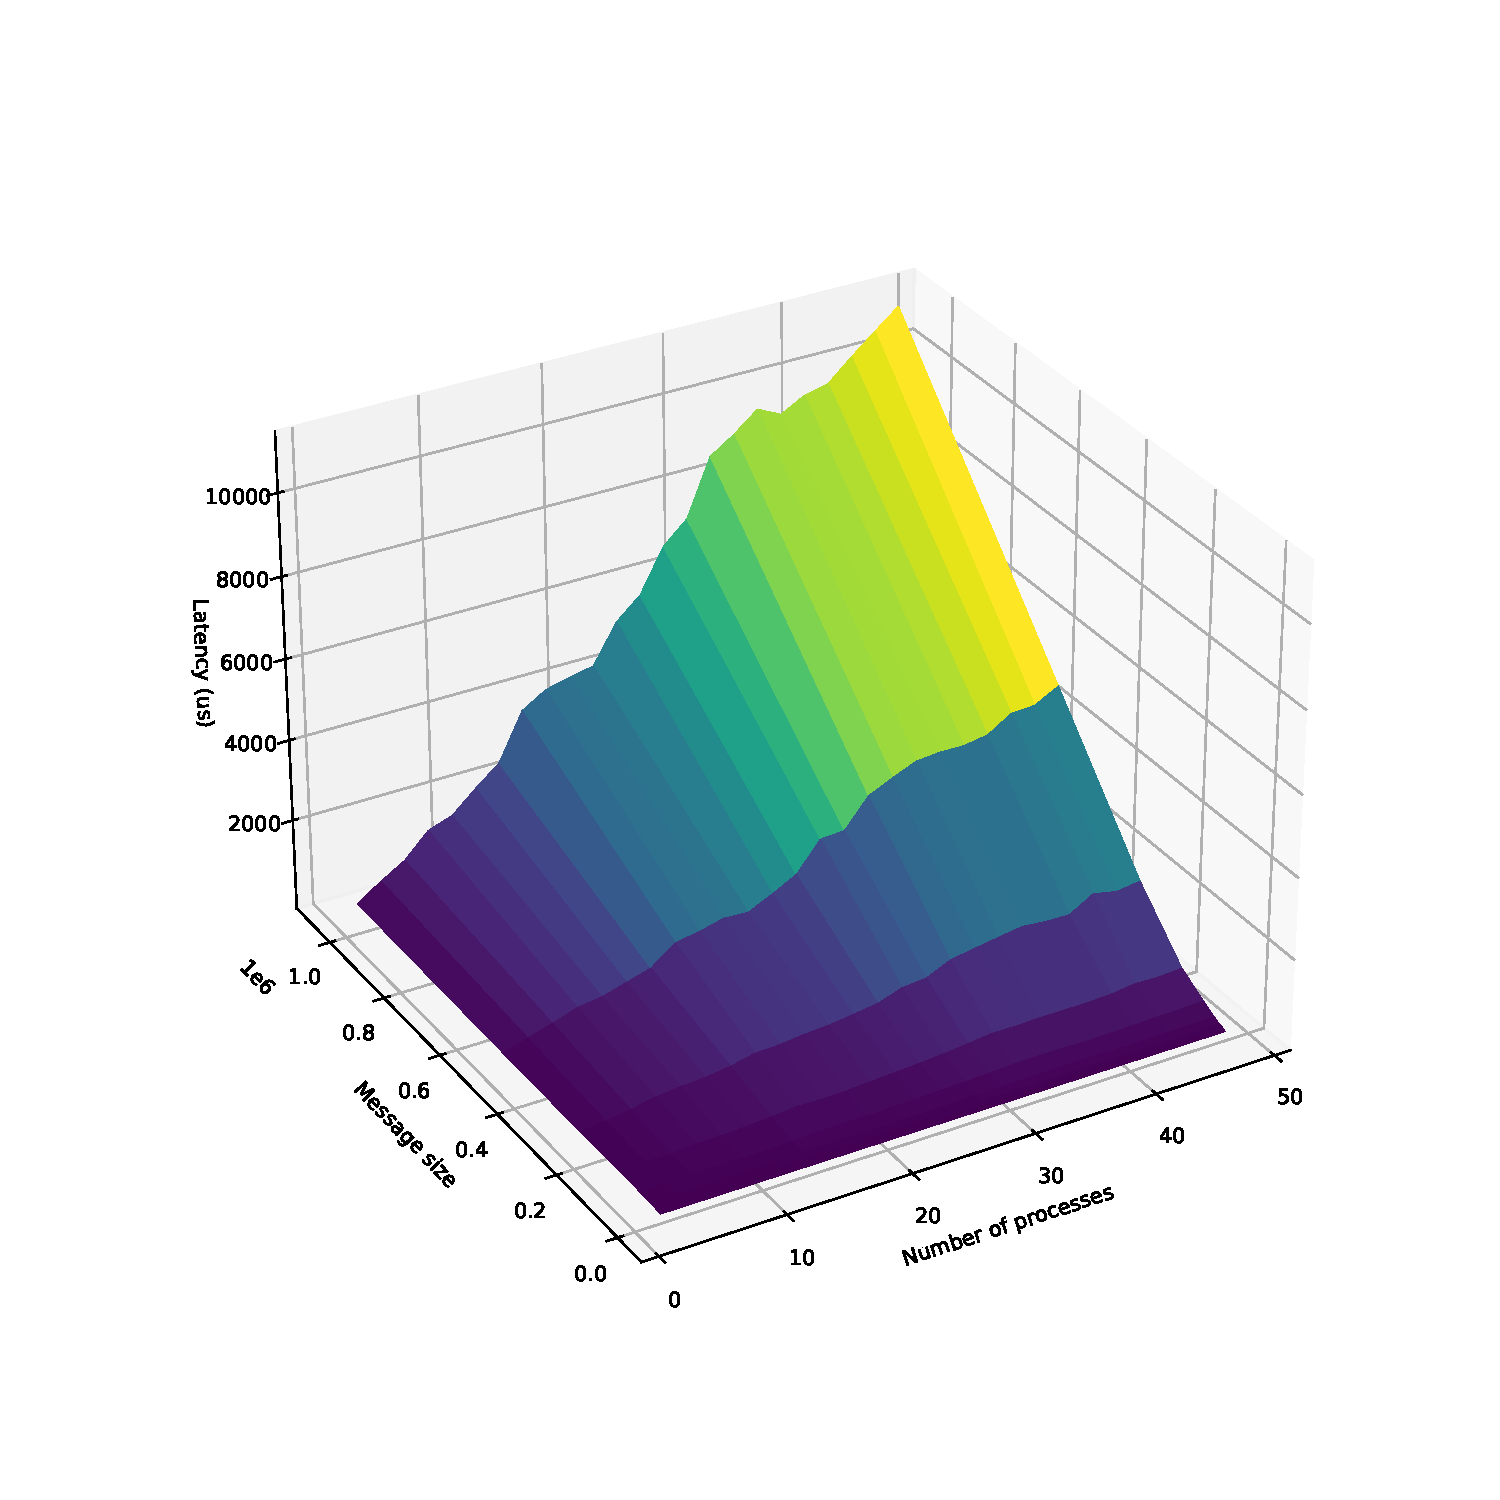
\includegraphics[
            width=0.45\textwidth,
            clip,
            trim=0 3cm 0 4.5cm
        ]{figures/scat_node_alg2.pdf}
        \caption{Intra-Node scatter latency (binomial)}
    \end{figure}
\subsubsection{Intra-Cluster}
    Mapping by node, we perform the scatter operation between multiple
    processes on different nodes. The average latencies are reported in
    plot below.
    % Basic Linear
    \begin{figure}[H]
        \centering
        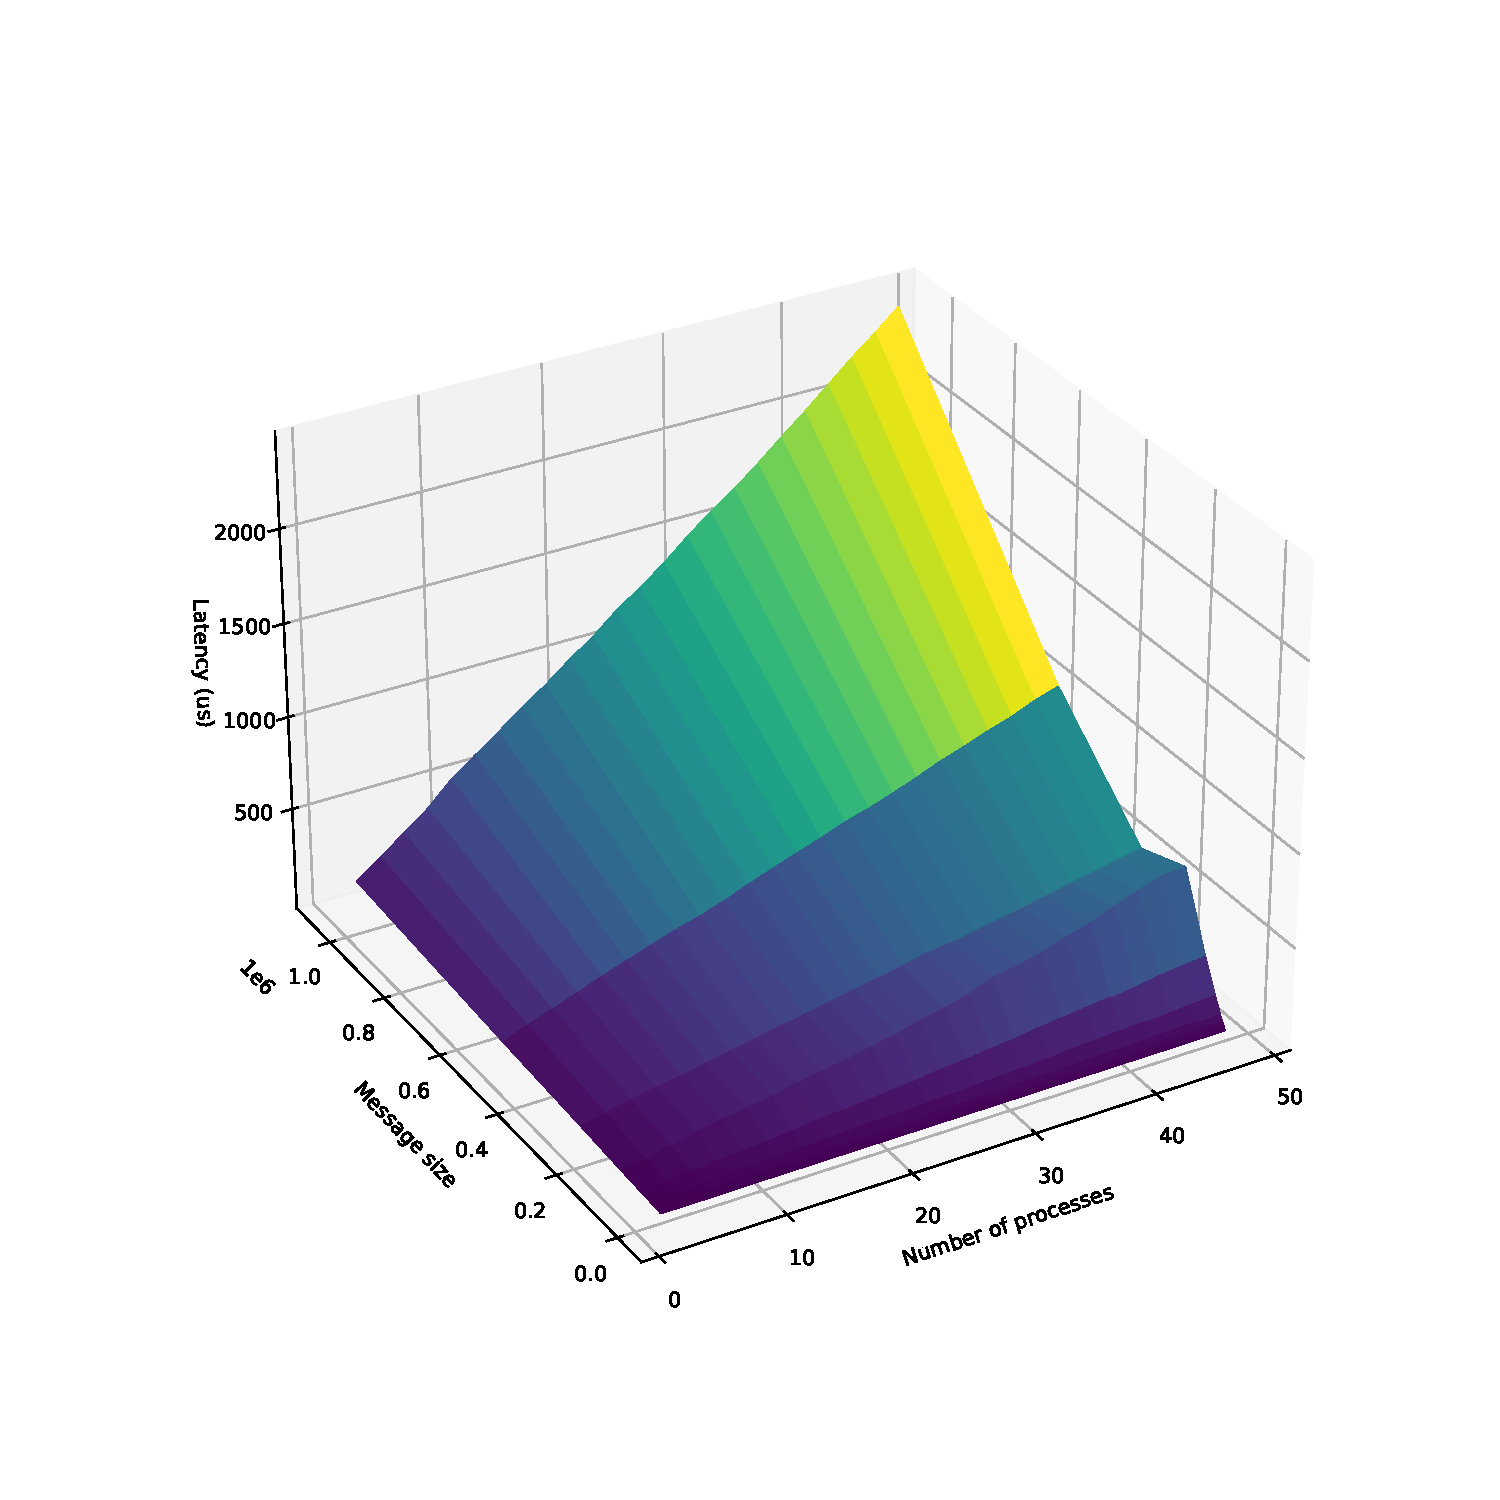
\includegraphics[
            width=0.45\textwidth,
            clip,
            trim=0 3cm 0 4.5cm
        ]{figures/scat_cluster_alg1.pdf}
        \caption{Intra-Cluster scatter latency (basic linear)}
    \end{figure}
    % Binomial
    \begin{figure}[H]
        \centering
        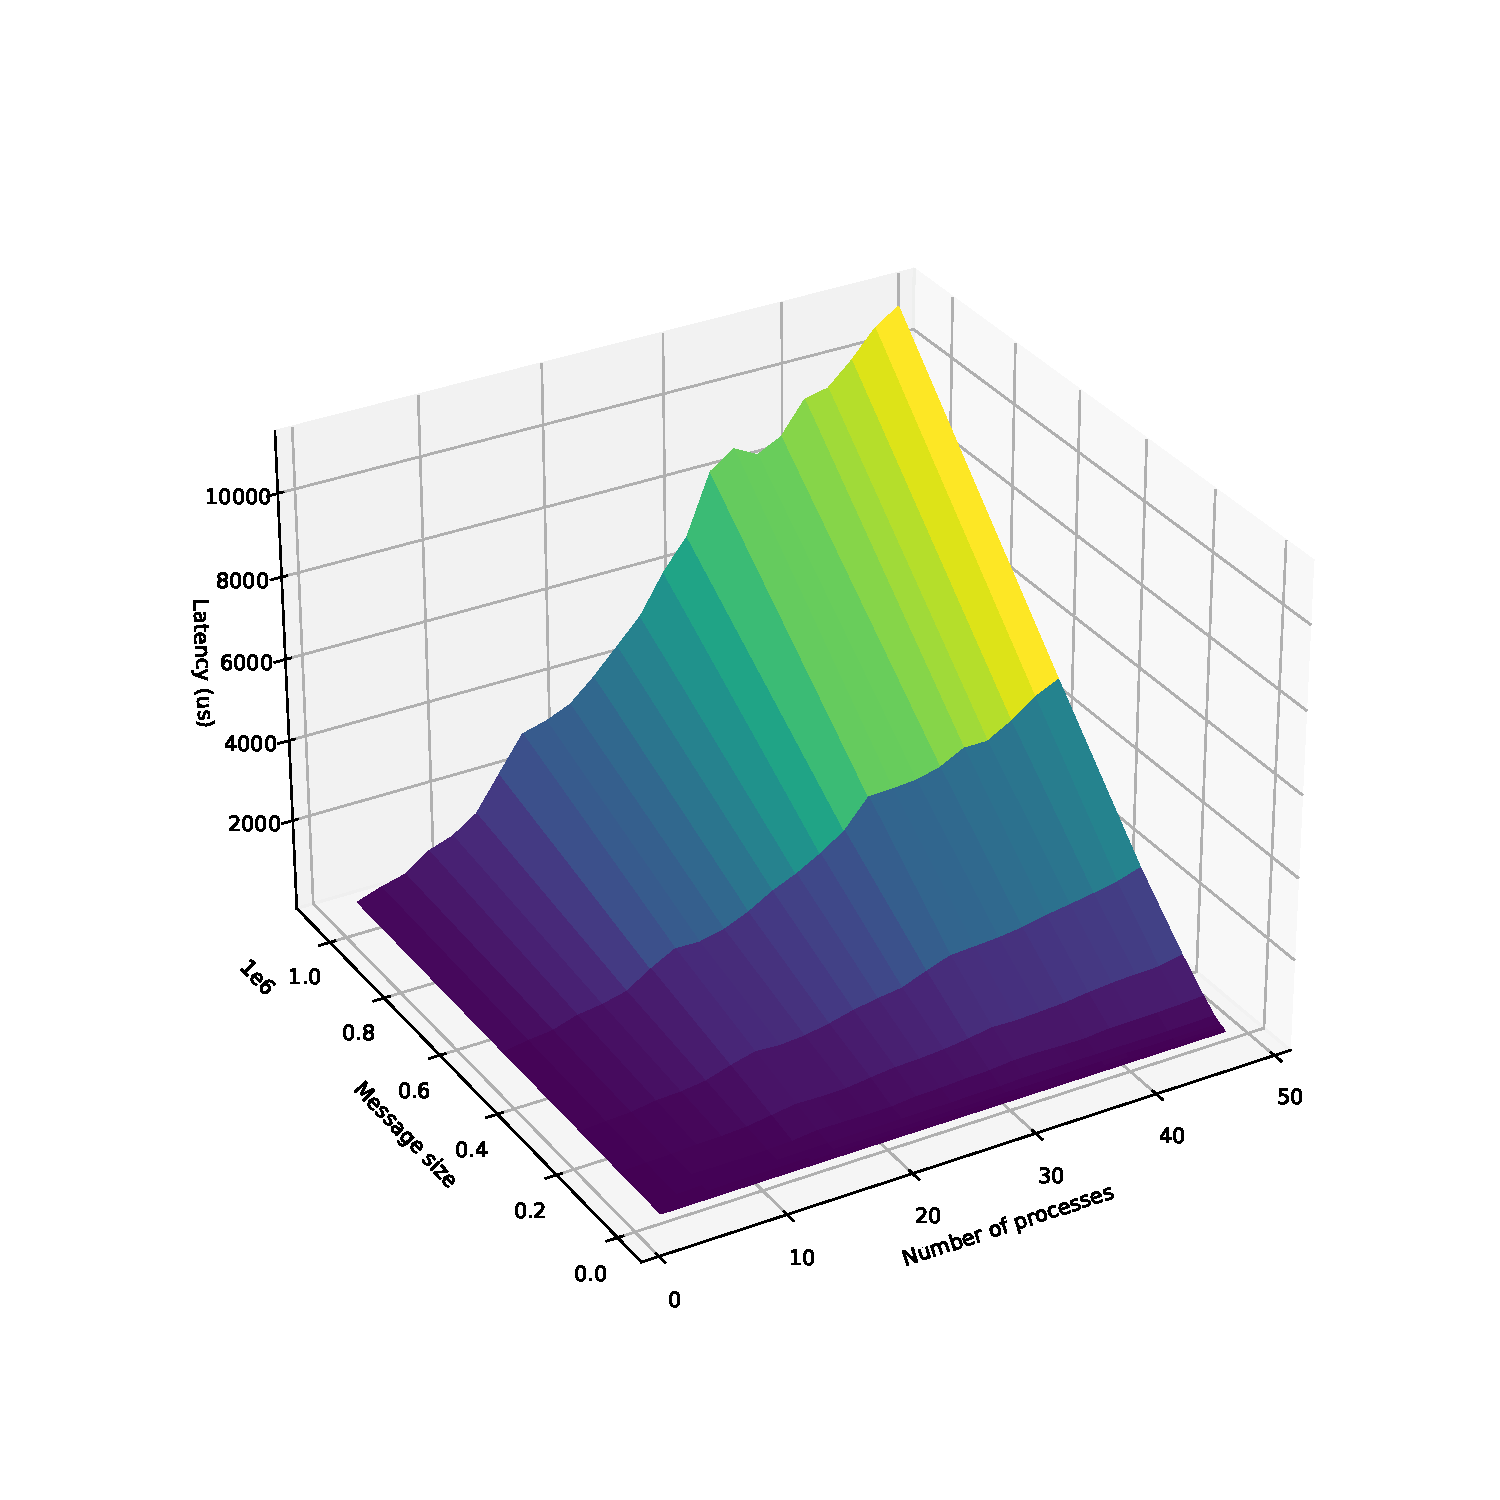
\includegraphics[
            width=0.45\textwidth,
            clip,
            trim=0 3cm 0 4.5cm
        ]{figures/scat_cluster_alg2.pdf}
        \caption{Intra-Cluster scatter latency (binomial)}
    \end{figure}    



